\documentclass[b5paper,12pt,dvipdfmx]{jsreport}
\usepackage[top=2cm,bottom=2cm,left=2.5cm,right=2.5cm]{geometry}

\usepackage{bm}
% \usepackage[dvipdfmx]{graphicx}
\usepackage{ascmac}

% 画像読み込みよう
\usepackage[dvipdfmx]{graphicx}

\usepackage{caption}


\usepackage[dvipdfmx]{graphicx}
\usepackage[dvipdfmx]{color}

% \usepackage{color}
\newcommand{\red}[1]{\textcolor{red}{#1}}

\usepackage{booktabs}
\usepackage{adjustbox}

\usepackage{url}

\usepackage{indentfirst}

\usepackage{chngcntr}
\counterwithout{figure}{chapter}
\counterwithout{table}{chapter}

\usepackage{float}
 

% \usepackage[dvipdfmx]{graphicx}
% \usepackage[dvipdfmx]{color}


\setlength{\parskip}{2mm} % 3mmのスペースを挿入

% インデントを無効化
\setlength{\parindent}{0pt}


\title{多言語自動翻訳掲示板の利活用に関する実践研究}
\author{早稲田大学人間科学部人間情報科学科\\西村研究室\\ \\学籍番号:1J20F037\\名前:奥村飛悠}
\date{\today}
\renewcommand{\bibname}{参考引用文献}

\begin{document}
\maketitle

\pagenumbering{gobble} % 目次のページ番号を完全に消去
\tableofcontents

\clearpage % 新しいページを開始
\pagenumbering{arabic} % 本文のページ番号をアラビア数字に設定し,1から開始
\chapter{はじめに}
 
\section{現状}

インターネットの普及やソーシャルメディアの台頭により,オンラインでのコミュニケーションが一般的になっている(大向,2006).その中でも,誰でも気軽に参加することのできる掲示板は重要なコミュニケーションの場となっている.日本では,"5ちゃんねる"(サイト名を"2ちゃんねる"から"5ちゃんねる"へ2017年10月に変更)が広く知られている一方で,米国発の"reddit"は国際的に認知度が高く,日別のアクティブユーザー数は5700万人,総投稿数は130億投稿を超えている(Reddit Inc,2023).これらの大規模な掲示板は情報の集積場所として,またユーザー間の活発な議論の場として重要な役割を果たしている.

しかしながら,掲示板は誰もが利用できるコミュニケーションの場であるにも関わらず,現状ではそのコミュニケーションは主に同一言語間で行われている.具体的には,"5ちゃんねる"では主に日本語,"reddit"では主に英語が使用されている.そのため,異なる言語を使用するユーザーは,翻訳ツールや外部の翻訳サービスを頼るか,専用のスレッドや言語コミュニティを探すことが一般的となっている.しかし,これらの方法にはデメリットが存在する.例えば,翻訳ツールを利用すると時間と手間がかかるため,掲示板の持つ即時性や気軽さというメリットを十分に享受することが難しくなる.

同一言語間でのコミュニケーションが主流となっている背後には複数の要因が考えられるが,その一つとして翻訳技術の品質が十分でなかったことが考えられる.2004年には「コミュニケーションツールとして使用する場合に十分な品質を持っているとはいい難い」(船越ほか,2004)との指摘があり,さらに2010年にも「近年,翻訳技術は急速に進展しているが,高精度な翻訳を行うことは困難である.コミュニケーションにおいて,不適切な翻訳箇所を含む文章は話者間の相互理解を困難にし,円滑なコミュニケーションの妨げとなる」(宮部ほか,2010)とも指摘されている.また,多言語間でのコミュニケーションにおいては,翻訳の品質が極めて大きな影響力を持つことも確認されている(船越ほか,2004).このように,コミュニケーションに大きな影響を与える翻訳技術の品質が十分でなかったため,ユーザーは翻訳技術を利用して会話の中心となっている言語以外を使用してまで会話を試みなかったのではないだろうか.


\section{翻訳技術の進歩}

しかしながら,翻訳サービスの精度は日々向上している.これについて,「近年,Google翻訳やDeepL,そしてページ全体翻訳機能の進化が著しい」(村本,2022)との報告があり,その背景には機械学習の進歩が影響を与えている.「Google英日翻訳がNMT(ニューラル機械翻訳)を採用したことで,目標言語の流暢さが格段に向上した」(影浦,2017)との報告がある.同様にNMTを採用しているDeepLは,2017年にサービスを開始し,その高品質な翻訳サービスが評価されている(亀田,2022).さらに「2020年と2021年には,文章の意味をより正確に伝えられ,業界特有の専門用語もうまく処理できる新たなモデルを発表」(DeepL,2023)している.これらのことから,翻訳サービスの精度は日々向上されていることが分かる.

また,多くの翻訳サービスが開発者向けにAPIを提供している.その代表例としては,Google CloudのTranslation AI(Google Cloud,2023)やDeepL API(DeepL,2023)がある.これらのサービスを開発者が利用するための便利なライブラリも存在している.具体的には,Google Translate API(現在のTranslation AI)を利用するためのPythonのライブラリであるgoogletrans(PyPI,2023a)やdeepl(PyPI,2023b)がある.このようなAPIやライブラリの存在により,開発者は翻訳機能を自身のサービスに容易に組み込むことが可能となっている.

\section{既存サービスと先行研究}

過去には,"enjoy Korea"という日本語と韓国語の翻訳機能を持つ掲示板サービスが存在していたが,利用率の低下を理由に2009年6月8日にサービスを終了している(野津,2009).また,小川ら(2009)は日本語とウイグル語間の翻訳掲示板システムを開発している.しかし,彼らの研究は主にシステムの開発に焦点を当てており,システムを使用するユーザーのデータ収集やその分析までには至っていない.

一方,藤井ら(2005)はアノテーションや折り返し翻訳に着目し,中国語,韓国語,日本語間の翻訳BBSである"AnnoChat"を開発した.翻訳の精度がコミュニケーションの理解度に影響を与える可能性を示しているが,ユーザー同士の具体的なコミュニケーションの内容までは調査していない.また,吉野ら(2006)はユーザインタフェースのカスタマイズ性に焦点を当てた研究を行い,"CustomChat"というシステムを開発したが,これも具体的なチャットの内容などについては触れられていない.

これらの事例や研究を見ると,多言語間のコミュニケーションを可能にする翻訳掲示板に関する研究やサービスは確かに存在している.しかし,それらは主にシステムの開発や翻訳の精度と理解度の関係性,ユーザインタフェースの改良に焦点を当てており,異なる言語を使用するユーザーがシステムをどのように使うのか,どのようなコミュニケーションが起こるのかという点については,まだ十分に研究されていないと言える.


\section{本研究の概要と目的}

これらの背景から,本研究では,掲示板のグローバル化を進めるため,近年の高精度な翻訳サービスを利用した多言語自動翻訳掲示板の開発とその利活用について実践的な研究を行う.我々が提案する多言語自動翻訳掲示板では,ユーザーは表示言語を選択することにより,選択した言語で掲示板の投稿を閲覧することを可能にする機能をつける.これにより,異なる言語を使用するユーザー間でも,自由なコミュニケーションが促進され,掲示板の持つ即時性や気軽さというメリットを維持することができる.

そして,この掲示板をインターネット上に公開し,使用者から得られるデータを収集する.その後,得られたデータを分析し,多言語自動翻訳掲示板がユーザーのコミュニケーションにどのような影響を与えるのか,多言語自動翻訳掲示板上で異なる言語を使用するユーザー同士がどのようなコミュニケーションをするのかを評価する.具体的には,ユーザー間のコミュニケーション量や内容,トピックの多様性,言語間のコミュニケーション方法などを指標として用いる.

我々の研究は,新たな掲示板の形を示すだけでなく,機械翻訳技術とその実用化の進歩に貢献することを期待している.本研究の結果が,ユーザーが自由に多言語コミュニケーションを享受できるインターネットの環境整備に向けた一歩となることを願っている.


\chapter{多言語自動翻訳掲示板について}


\section{システムの概要}

本研究では,多言語自動翻訳掲示板である「The Channel」というWebアプリケーションを開発した.このシステムは,世界中のユーザーが自分の言語で投稿することができる.そして,その投稿は閲覧するユーザーが選択した言語に翻訳されて表示されるため,ユーザーは好きな言語でコンテンツを読むことができる.

システムの中核は,機械翻訳技術が担っている.これにより,ユーザーが投稿したテキストはリアルタイムで他の言語に翻訳され,多様なユーザーがアクセスできるようになる.例えば,日本語で書かれた投稿は,英語,スペイン語,中国語などに瞬時に翻訳され,異なる言語のユーザー間の交流を可能にする.

システムは,掲示板として必要最低限の機能を備えている.ユーザーは簡単にスレッドを作成することや,自分の母国語でコメントを投稿することができる.

セキュリティに考慮し,ユーザーの個人名やメールアドレス等を取り扱わないようにしている.


\section{主な機能と利用フロー}

掲示板は以下の機能を持つ.

- スレッド作成:新しいスレッドを作成する機能

- コメント投稿:既存のスレッドに対してコメントを投稿する機能

- 閲覧:スレッドの内容を表示する機能

- 言語選択:ユーザーが表示言語を選択する機能

図\ref{system_usage_flow}にシステム利用フローを示す.

(1)ユーザーはブラウザを通して掲示板を閲覧する.

(2)ユーザーは閲覧しているスレッドに対してコメントを投稿することができる.

(3)ユーザーは自由にスレッドを作成することができる.

(4)ユーザーはいつでも言語を選択することができる.

\begin{figure}[H]
	\centering
	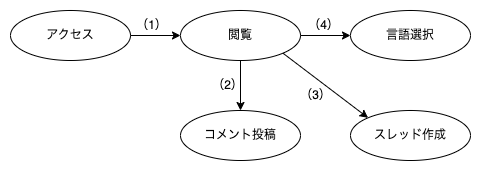
\includegraphics[width=124mm,height=45mm]{img/system_usage_flow.png}
	\caption{システム利用フロー}
    \label{system_usage_flow}
\end{figure}


\subsection{システムの画面}

以下に,主要な画面の概要を示す.


\subsubsection{トップページ画面}
トップページ画面(図\ref{fig:top_page})は,システムへの入口であり,ユーザーがスレッドを選択する主要な場である.この画面は,最新更新スレッドリストと新着スレッドリストが表示されている.任意のスレッドを選択することで,スレッドの中身を閲覧することができる.


\begin{figure}[H]
	\centering
    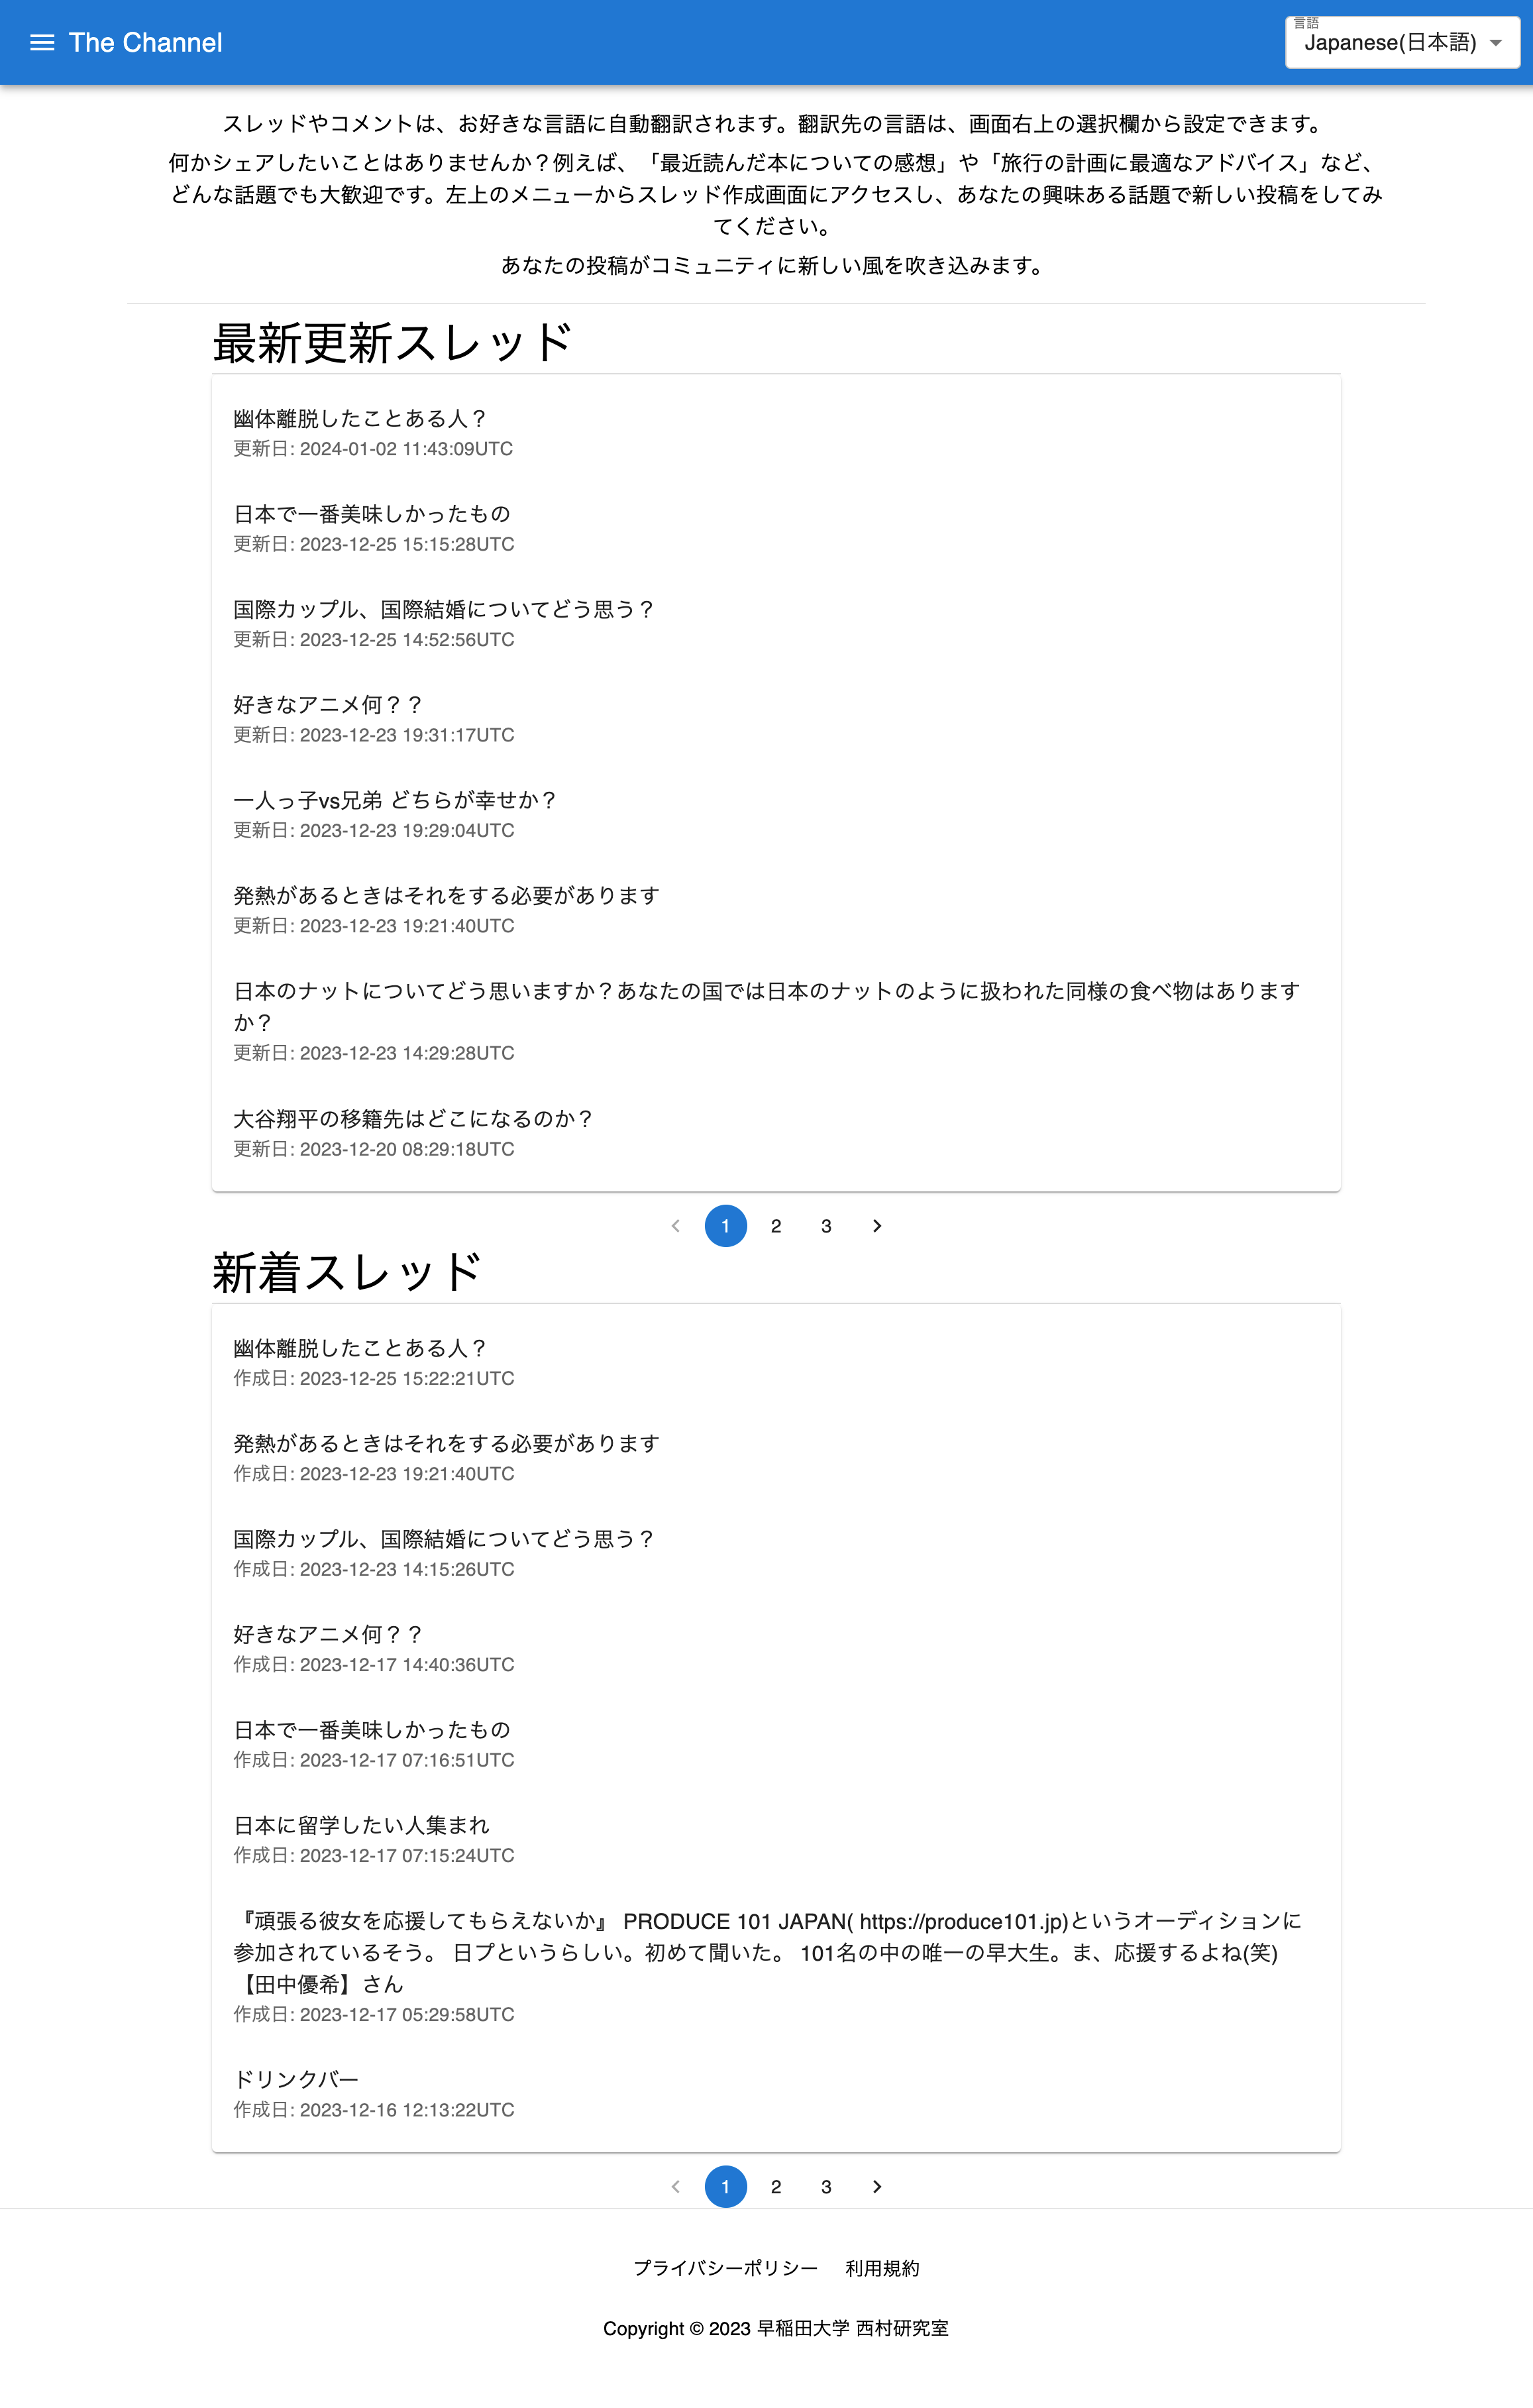
\includegraphics[width=100mm,height=157.04mm]{./img/screen/top_page.png}
	\caption{トップページ画面}
	\label{fig:top_page}
\end{figure}

\subsubsection{スレッド詳細画面}
スレッド詳細画面(図\ref{fig:thread_detail})では,選択されたスレッドの内容と,それに対するユーザーのコメントが表示される.ユーザーは,この画面の下部にある入力欄を使用して新たなコメントを投稿することが可能である.

\begin{figure}[H]
	\centering
    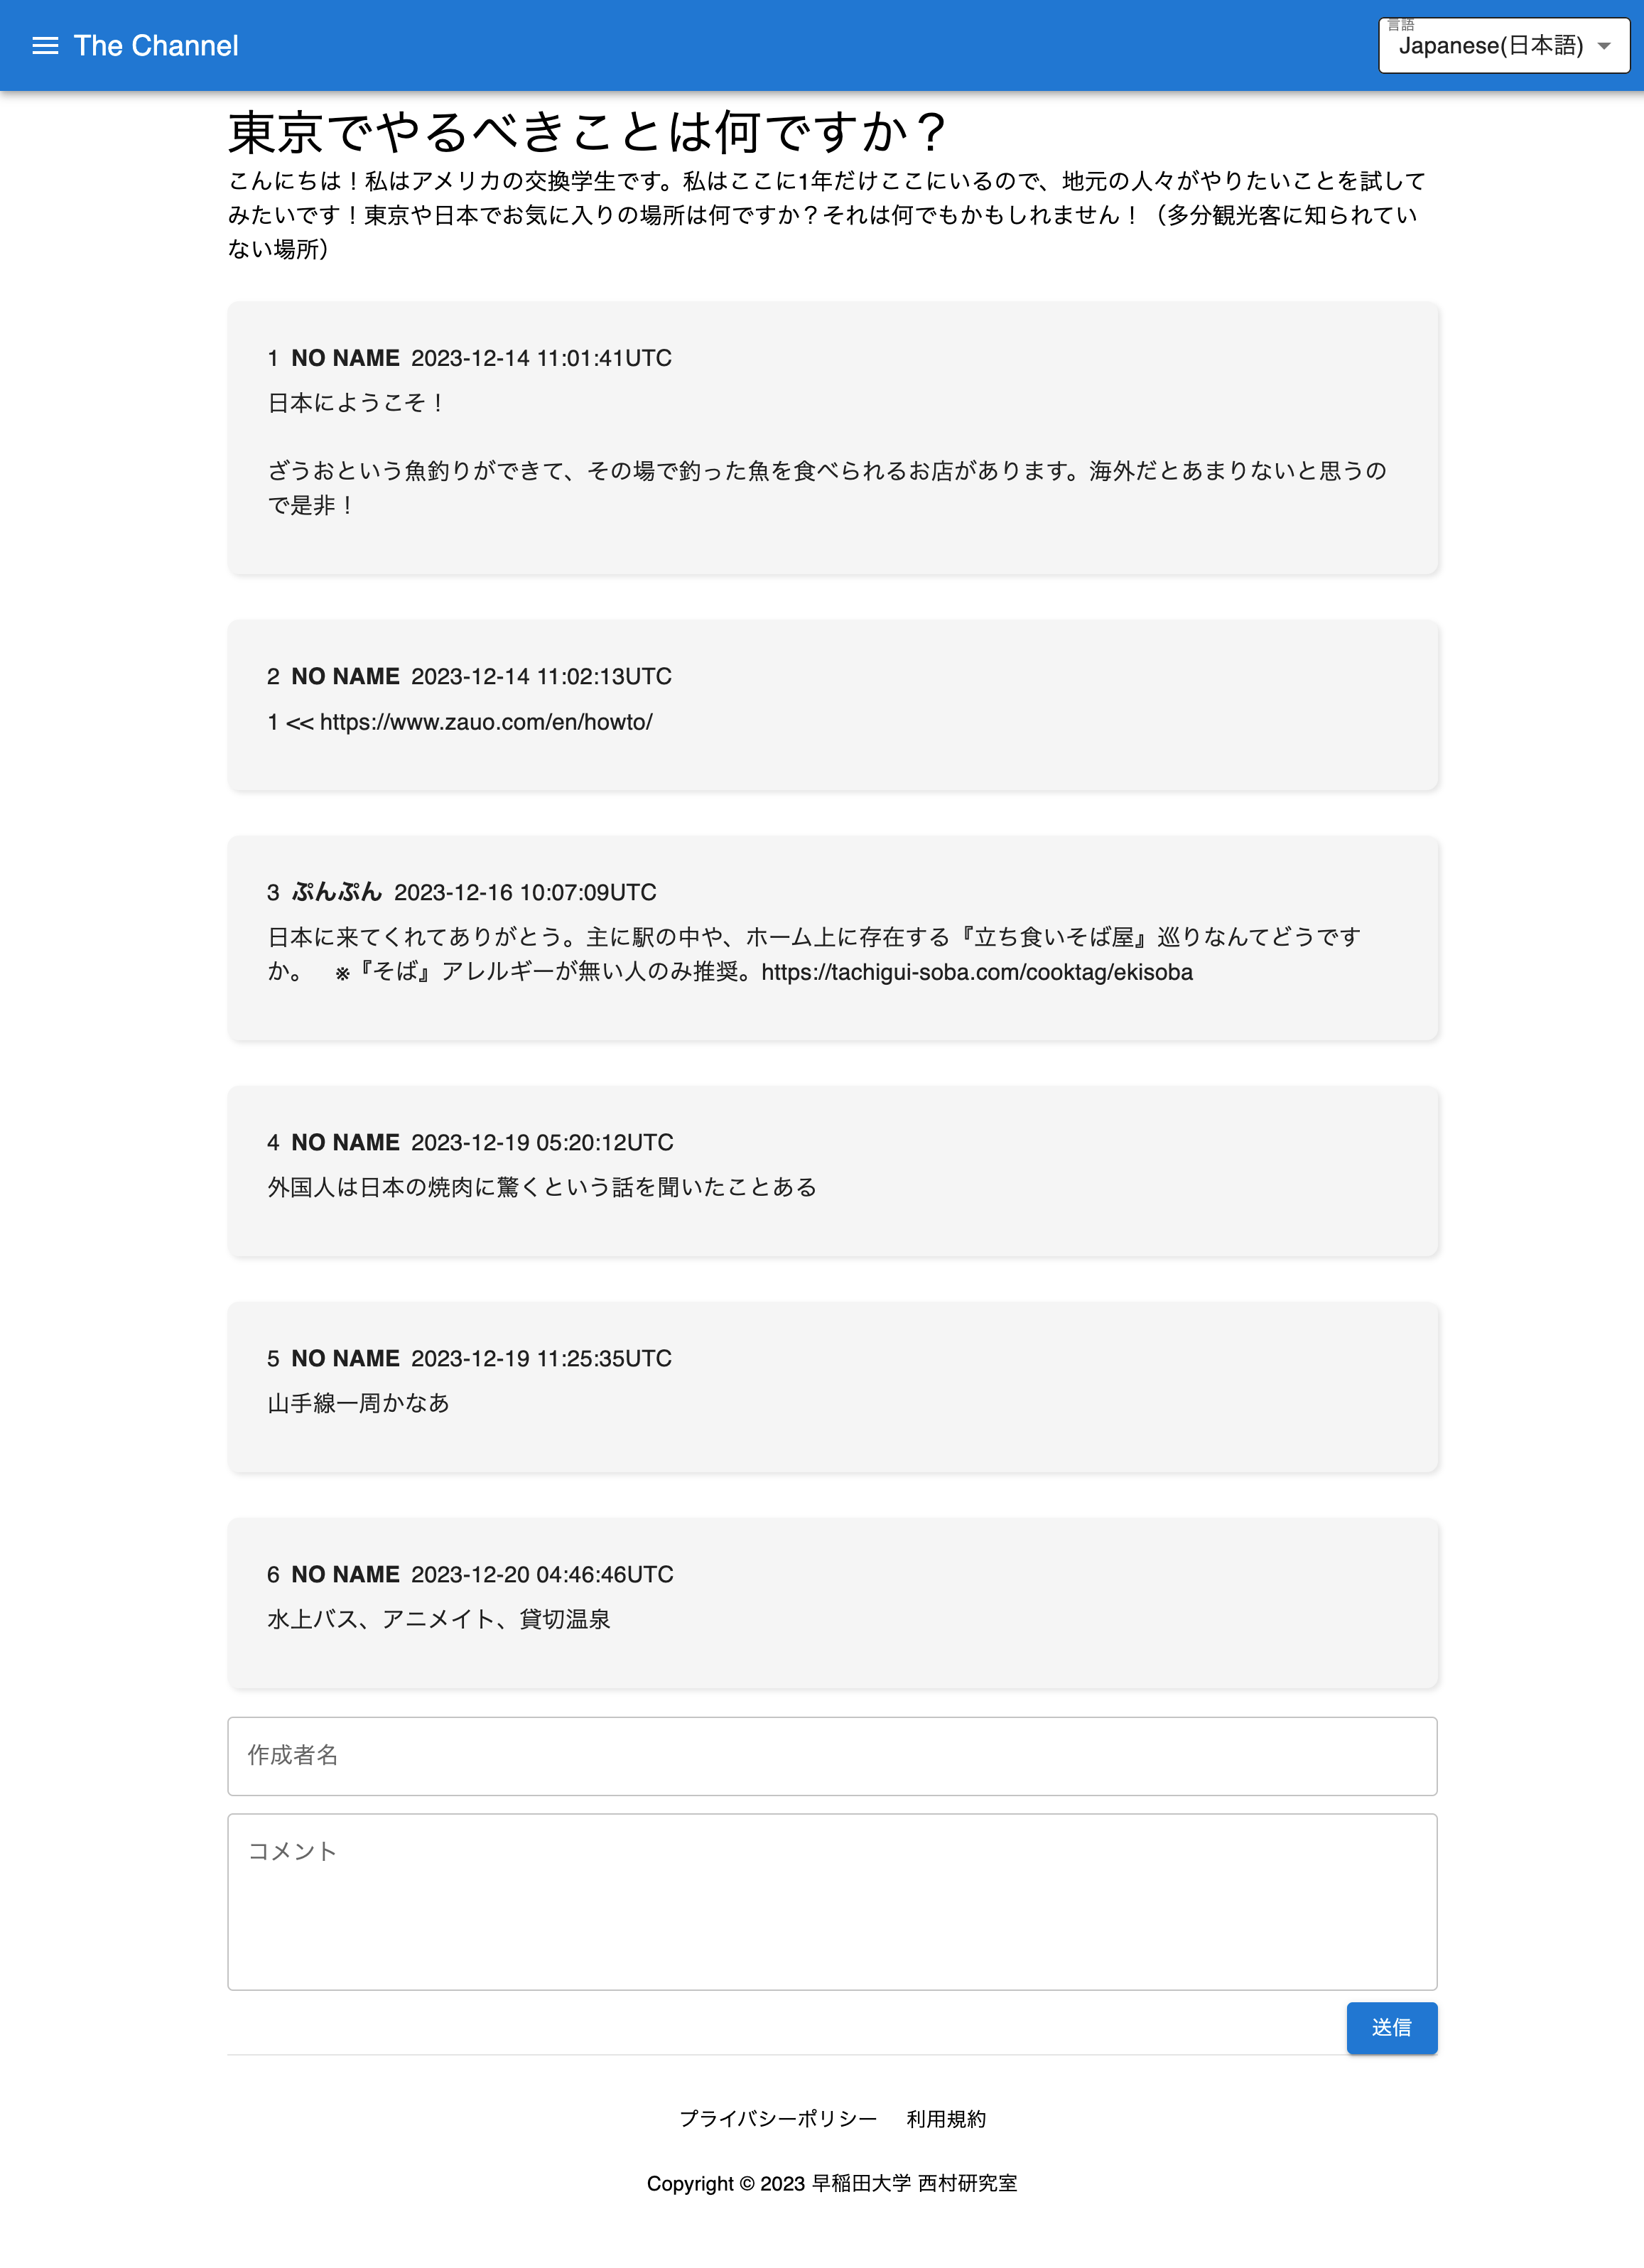
\includegraphics[width=100mm,height=137.94mm]{./img/screen/thread_detail.png}
	\caption{スレッド詳細画面}
	\label{fig:thread_detail}
\end{figure}


\subsubsection{スレッド作成画面}
スレッド作成画面(図\ref{fig:thread_create})では,ユーザーが新たなスレッドを作成することができる.

\begin{figure}[H]
	\centering
    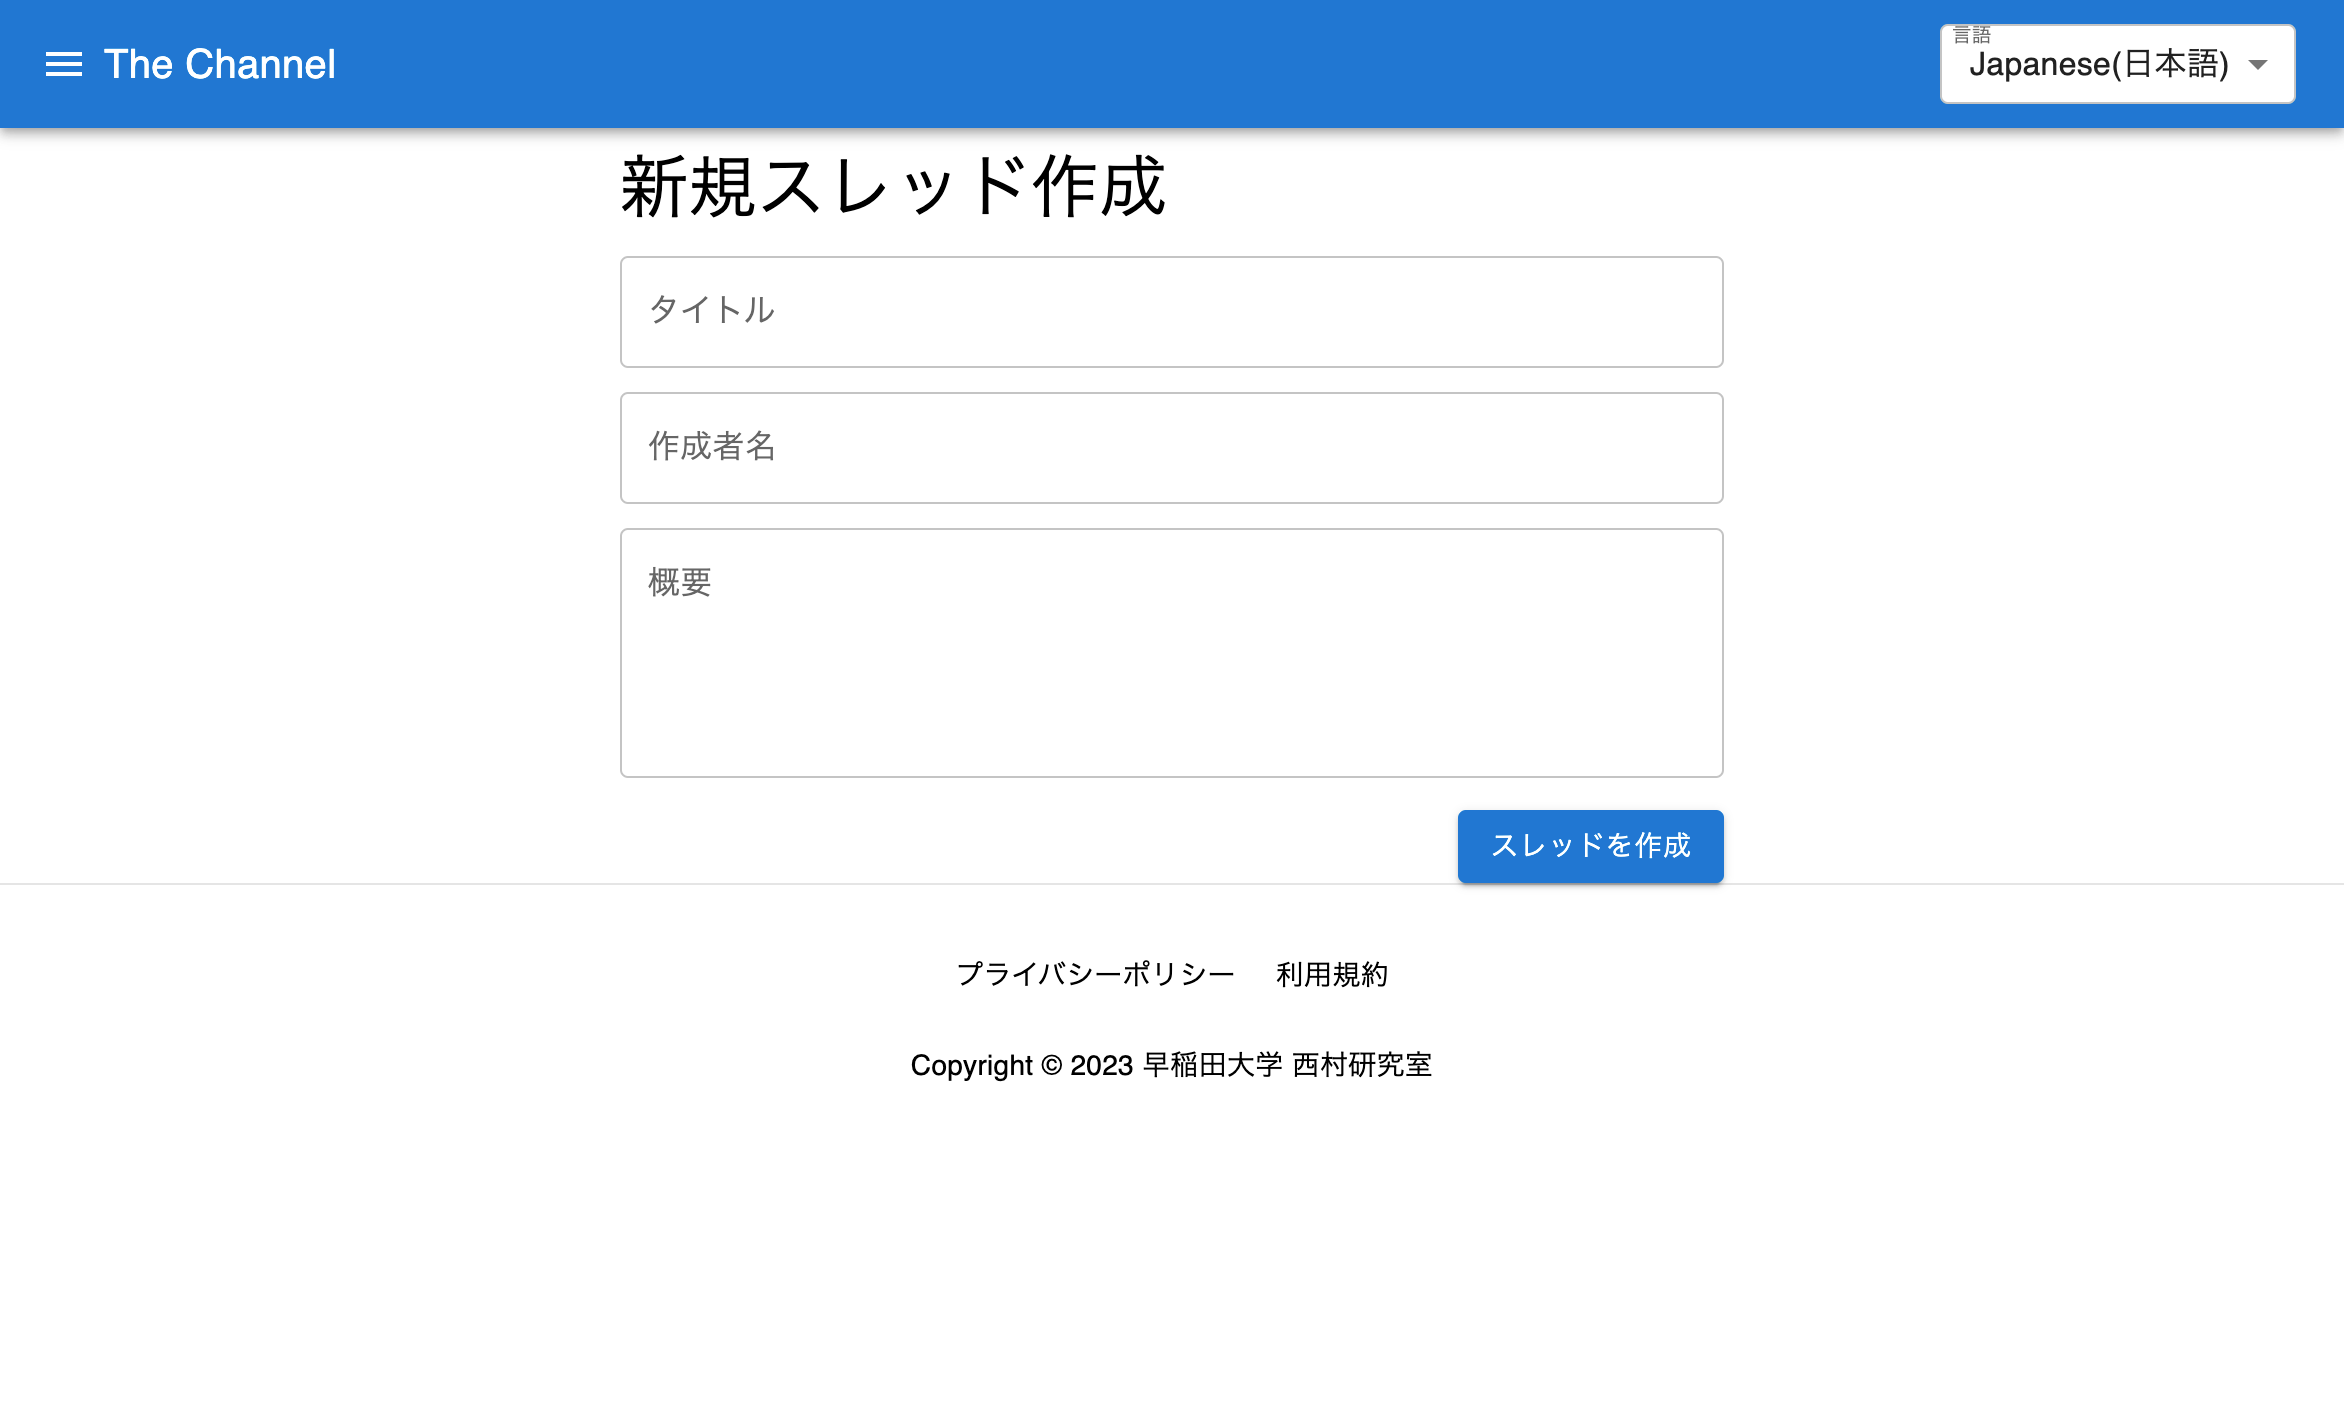
\includegraphics[width=100mm,height=60.67mm]{./img/screen/thread_create.png}
	\caption{スレッド作成画面}
	\label{fig:thread_create}
\end{figure}


\subsection{主要機能とその操作}

以下では,各機能の詳細と画面操作を説明する.


\subsubsection{スレッド作成}
スレッド作成画面(図\ref{fig:thread_create})では,新規のスレッドを作成することができる.スレッド作成欄(図\ref{fig:thread_textfield})にタイトルと作成者名と概要を入力し,「スレッドを作成」ボタンをクリックすることでスレッドが作成される.空欄の場合にはエラーが表示される(図\ref{fig:thread_textfield_error}).

\begin{figure}[H]
	\centering
    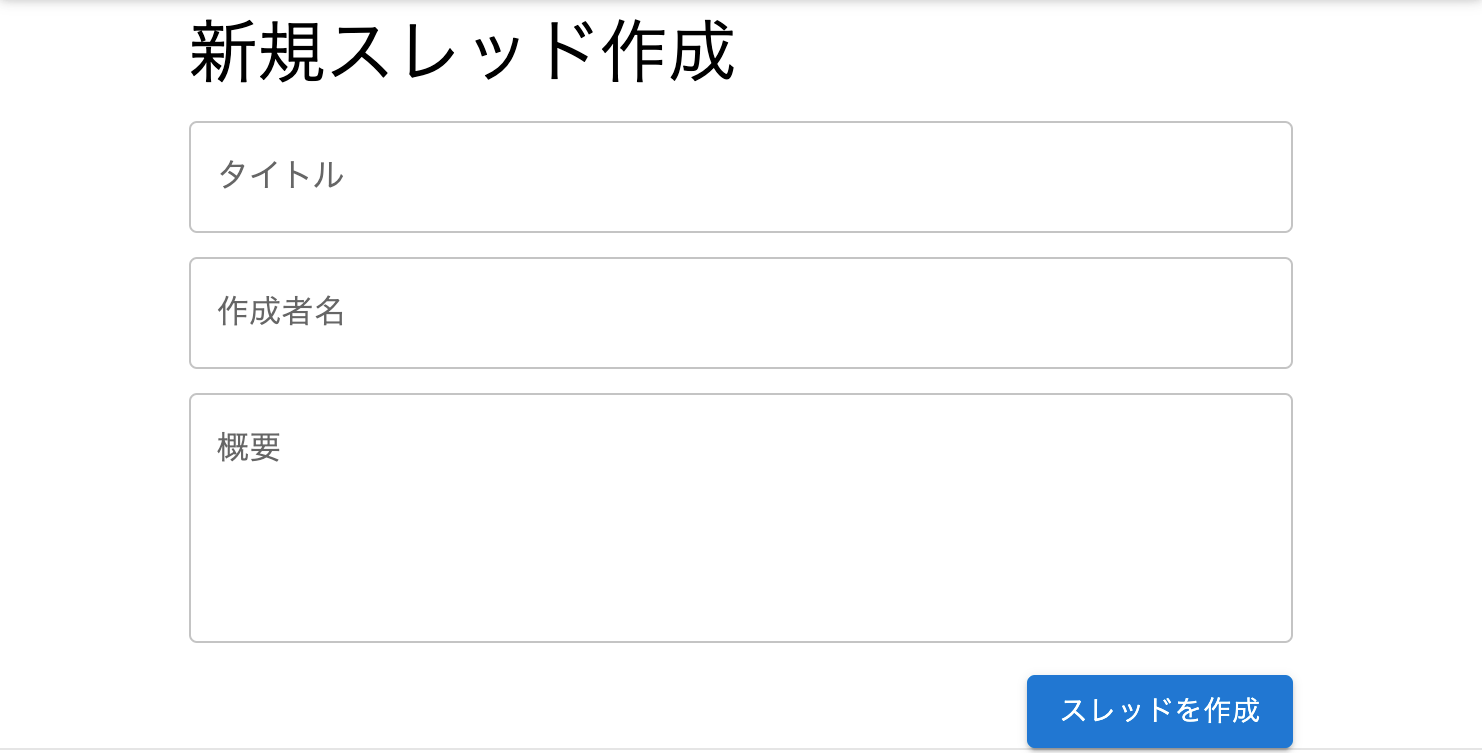
\includegraphics[width=100mm,height=50.81mm]{./img/feature/thread_textfield.png}
	\caption{スレッド作成欄}
	\label{fig:thread_textfield}
\end{figure}

\begin{figure}[H]
	\centering
    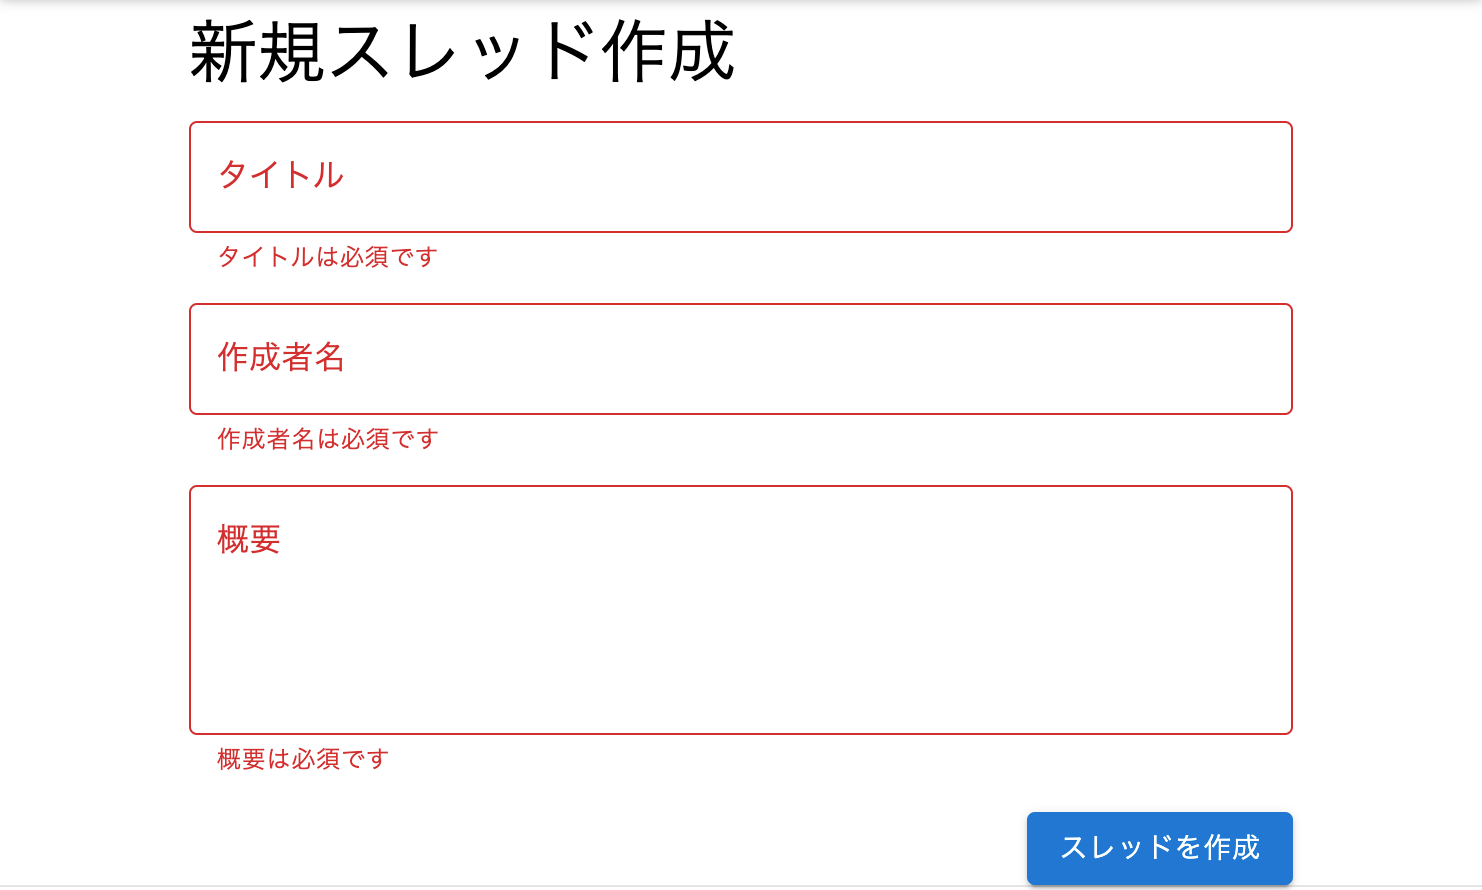
\includegraphics[width=100mm,height=60.05mm]{./img/feature/thread_textfield_error.png}
	\caption{スレッド作成欄エラー}
	\label{fig:thread_textfield_error}
\end{figure}

\subsubsection{コメント投稿}
スレッド詳細画面(図\ref{fig:thread_detail})では,既存のスレッドに対してユーザーはコメントを投稿することができる.コメント投稿欄(図\ref{fig:comment_textfield})に作成者名とコメント内容を入力し,「投稿」ボタンをクリックすることでコメントが投稿される.匿名投稿が可能である.コメントが空欄の場合にはエラーが表示される(図\ref{fig:comment_textfield_error}).

\begin{figure}[H]
	\centering
    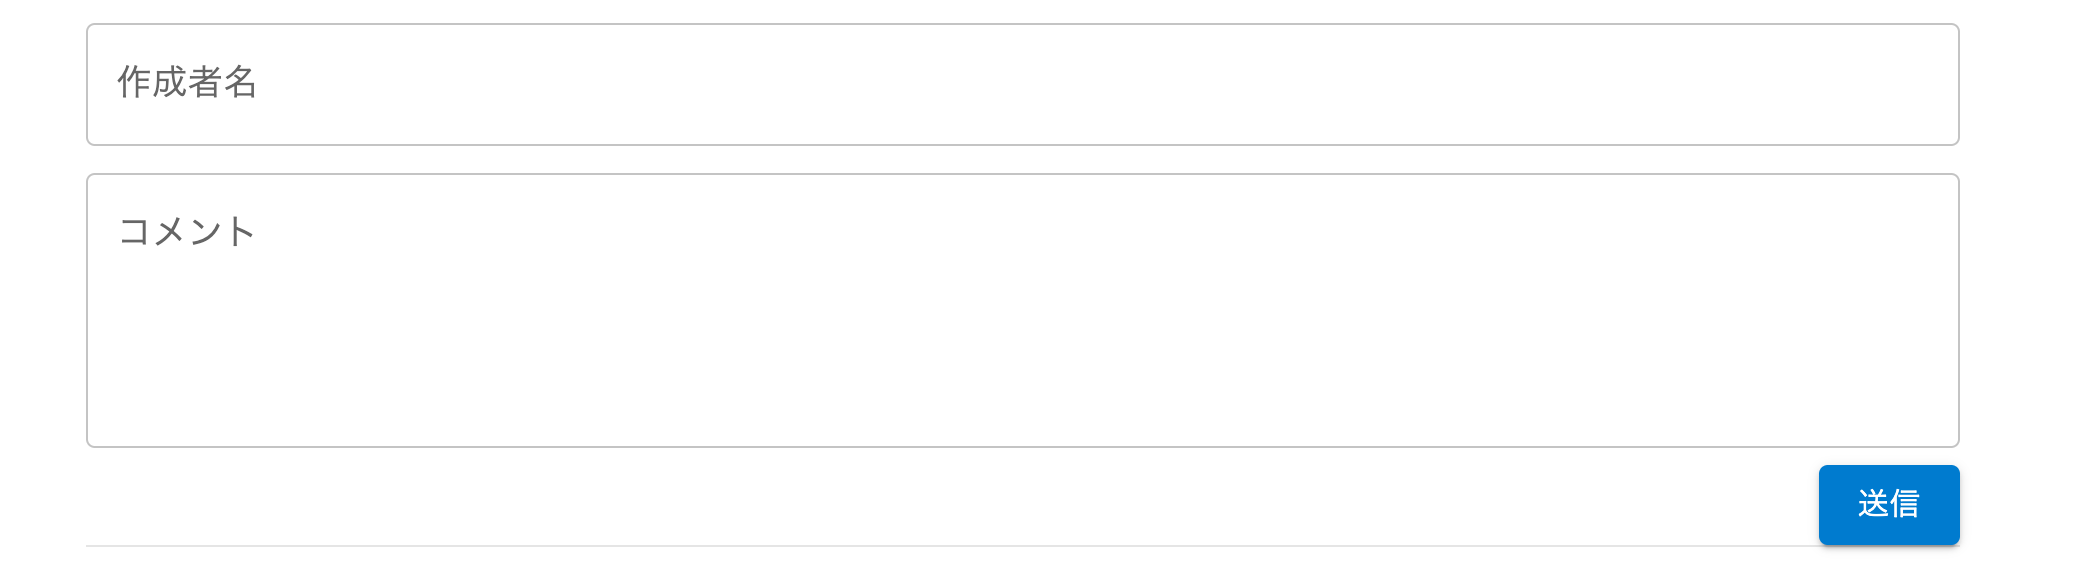
\includegraphics[width=100mm,height=28.19mm]{./img/feature/comment_textfield.png}
	\caption{コメント投稿欄}
	\label{fig:comment_textfield}
\end{figure}

\begin{figure}[H]
	\centering
    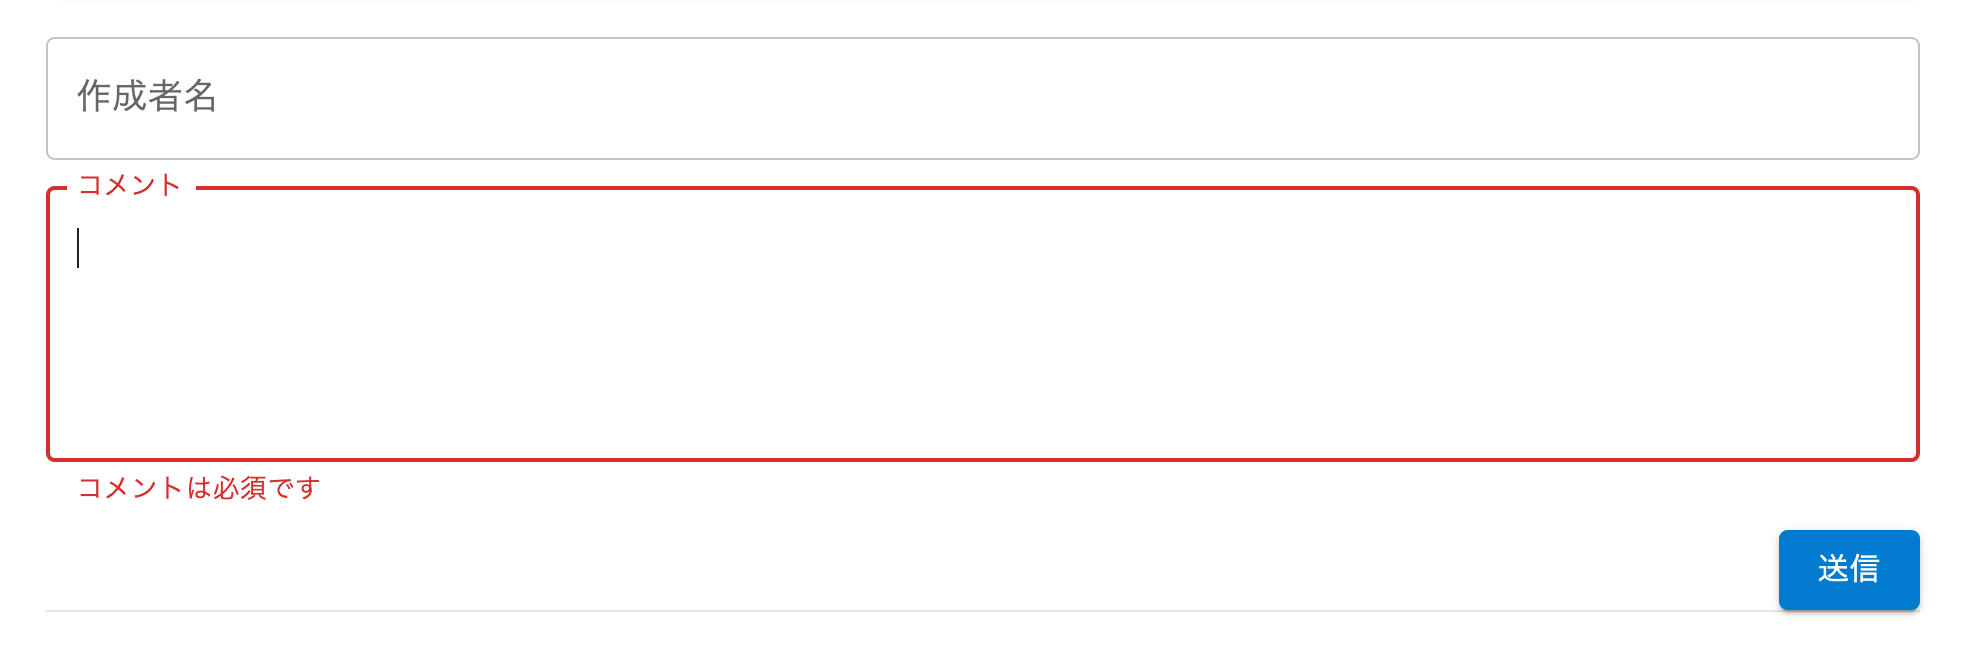
\includegraphics[width=100mm,height=32.90mm]{./img/feature/comment_textfield_error.png}
	\caption{コメント投稿欄エラー}
	\label{fig:comment_textfield_error}
\end{figure}

\subsubsection{スレッド詳細の閲覧}
トップページ画面(図\ref{fig:top_page})に表示されている最新更新スレッドリスト(図\ref{fig:latest_update_thread_list})または新着スレッドリスト(図\ref{fig:new_thread_list})から任意のスレッドを選択し,中身を閲覧することができる.

\begin{figure}[H]
	\centering
    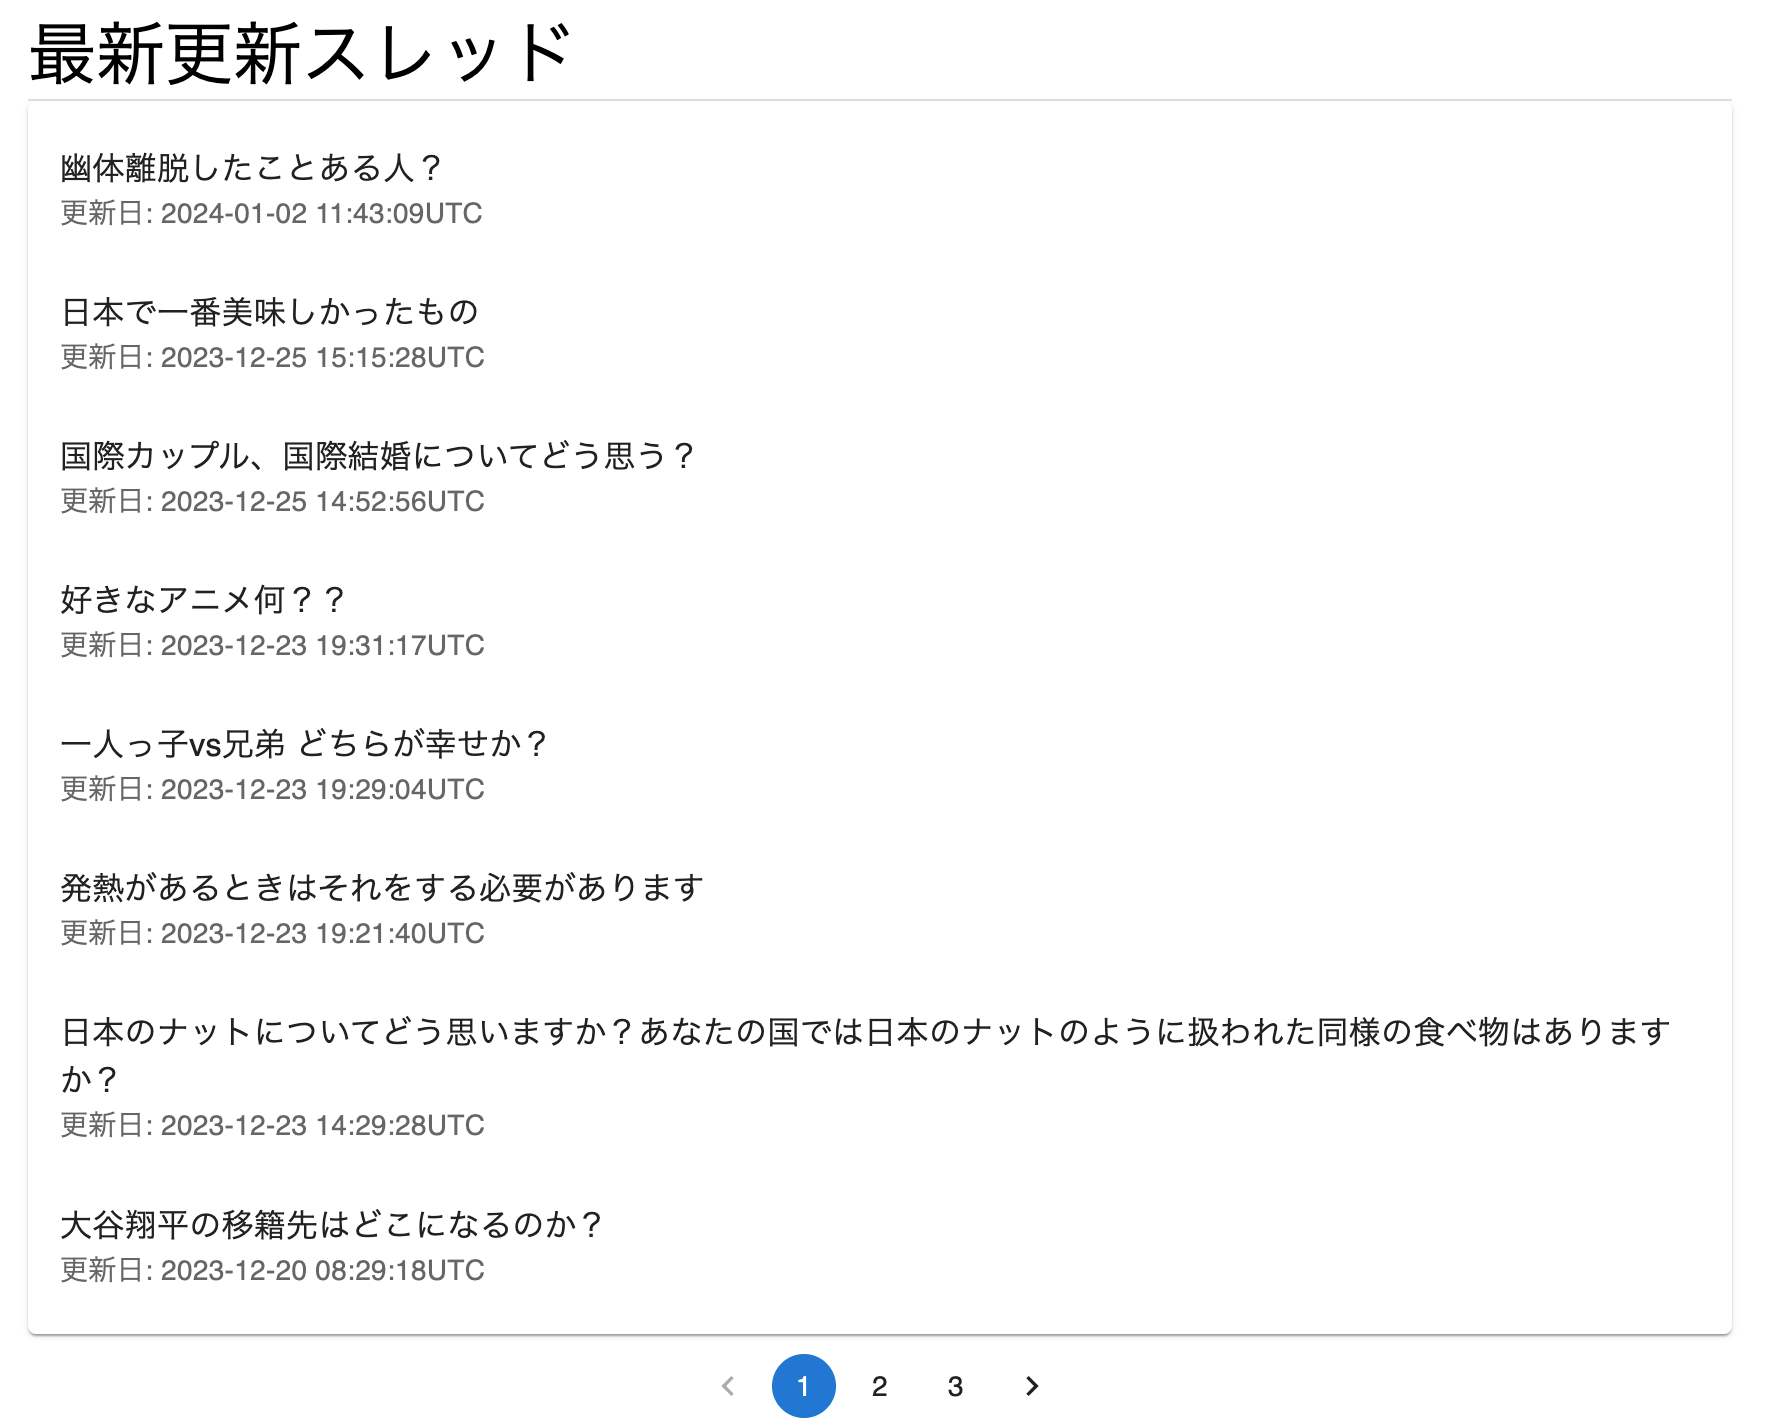
\includegraphics[width=100mm,height=79.79mm]{./img/feature/latest_update_thread_list.png}
	\caption{最新更新スレッドリスト}
	\label{fig:latest_update_thread_list}
\end{figure}

\begin{figure}[H]
	\centering
    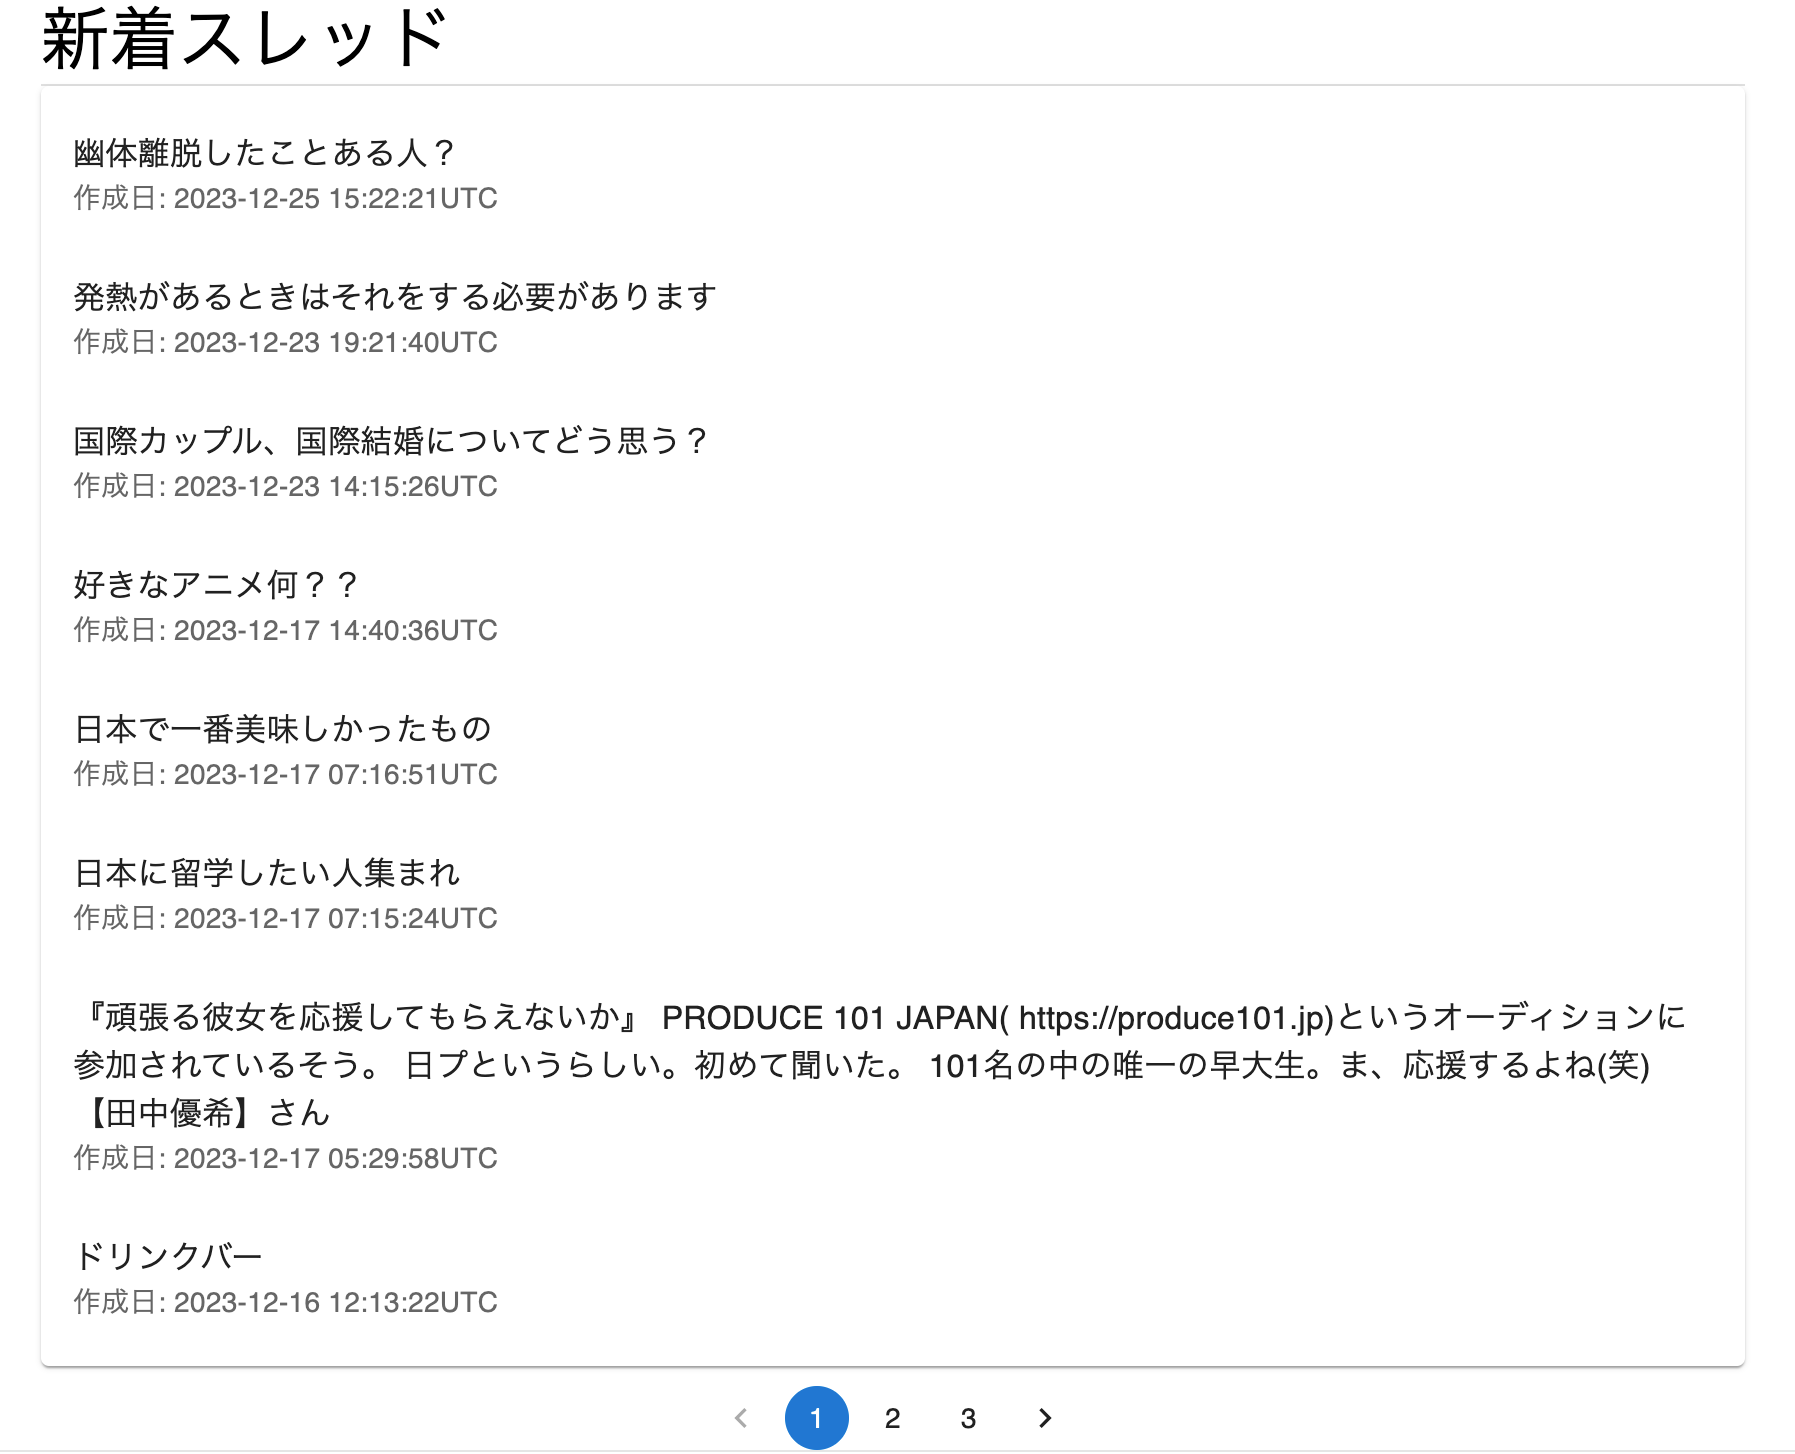
\includegraphics[width=100mm,height=81.00mm]{./img/feature/new_thread_list.png}
	\caption{新着スレッドリスト}
	\label{fig:new_thread_list}
\end{figure}

\subsubsection{ヘッダ}
ヘッダ(図\ref{fig:header})は,システム内のどの画面にいても常に上部に表示される.ヘッダには,サイトのロゴと言語選択メニュー,サイドメニューへのアクセスボタンが含まれている.

\begin{figure}[H]
	\centering
    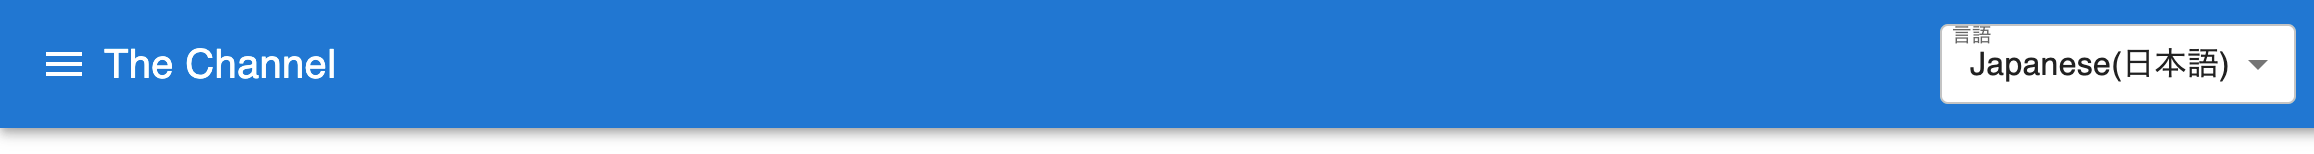
\includegraphics[width=100mm,height=6.66mm]{./img/feature/header.png}
	\caption{ヘッダ}
	\label{fig:header}
\end{figure}


\subsubsection{サイドメニュー}
サイドメニュー(図\ref{fig:side_menu})は,トップページとスレッド作成画面への遷移を提供する.ヘッダヘッダ(図\ref{fig:header})左部のメニューボタンをクリックすることで表示される.

\begin{figure}[H]
	\centering
    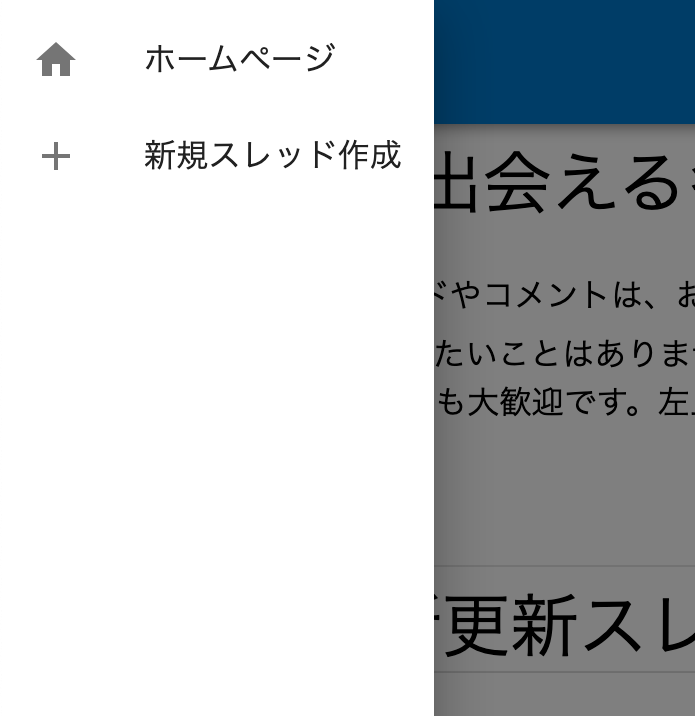
\includegraphics[width=100mm,height=103.02mm]{./img/feature/side_menu.png}
	\caption{サイドメニュー}
	\label{fig:side_menu}
\end{figure}


\subsubsection{言語選択}
ユーザーはヘッダー(図\ref{fig:header})に設置された言語選択欄(図\ref{fig:language_select})を通じて,掲示板の表示言語を自由に変更できる.この選択欄には言語がアルファベット順にリストされており,ユーザーは利用可能な言語の中から任意の言語を選択可能である.ここには,「Original」という特別な選択肢が用意されている.これを選択するとユーザーが入力した原文を翻訳せずにそのまま表示する.これにより,原文の内容をユーザーは確認することができる.また,「日本語」と「Original」は使用するユーザー数の多さを考慮してリストの先頭に配置されている.

% ユーザーは言語選択欄(図\ref{fig:language_select})から自由にシステムの表示言語を変更できる.ヘッダ(図\ref{fig:header})右部にある言語選択欄の利用可能な言語の中から選択する.選択された言語は,ユーザーが閲覧するコンテンツに適応される.言語は基本的にアルファベット順に並んでいる.ユーザー数が多い日本語とOriginalは先頭に表示した.Originalは言語として存在しているものではなく,本掲示板独自で追加したものである.これは,ユーザーが入力した文章を翻訳などをかけずにそのまま表示する設定である.

\begin{figure}[H]
	\centering
    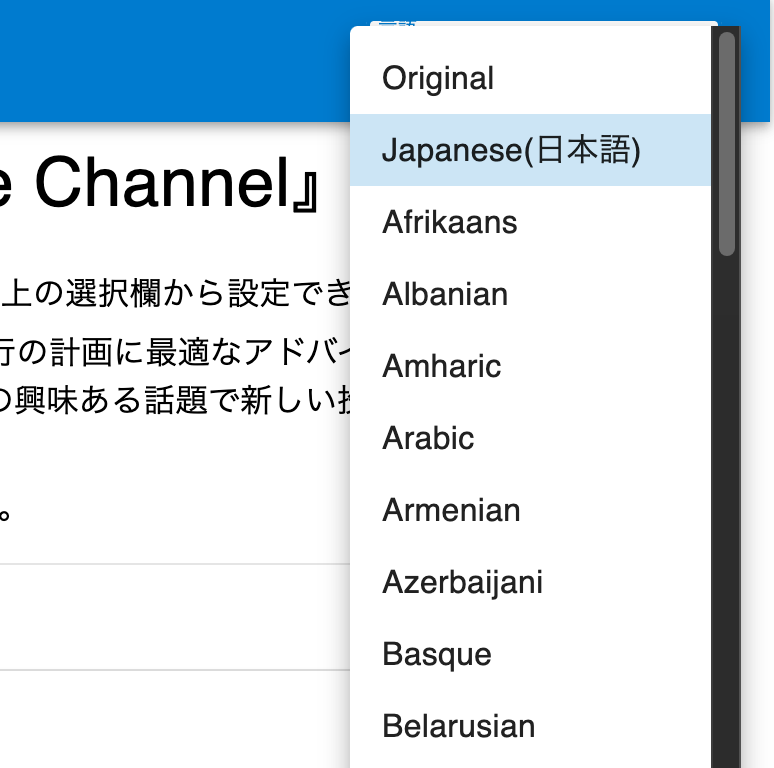
\includegraphics[width=100mm,height=99.22mm]{./img/feature/language_select.png}
	\caption{言語選択欄}
	\label{fig:language_select}
\end{figure}

% フッタには,システムの利用規約やプライバシーポリシーへのリンクが含まれており,ユーザーはこれらの文書に簡単にアクセスすることができる.また,フッタはシステム内のどの画面からでもアクセス可能であり,ユーザーに安心感を提供する.

\subsubsection{フッタ}
フッタ(図\ref{fig:footer})は,システム内のどの画面にいても常に上部に表示される.フッタには利用規約やプライバシーポリシーへのリンクが含まれており,ユーザーはこれらの文書にアクセスすることができる.

\begin{figure}[H]
	\centering
    
\includegraphics[width=100mm,height=17.33mm]{./img/feature/footer.png}
	\caption{フッタ}
	\label{fig:footer}
\end{figure}


\section{システム構成の概要}
開発した多言語自動翻訳掲示板は,フロントエンド,バックエンド,データベース,およびWebサーバーといった要素によって構成されている.図\ref{fig:tech_stack}にそれぞれの要素において採用した主要な技術を示す技術スタック図を示す.フロントエンドの開発には言語としてTypeScript,ライブラリとしてReact,フレームワークとしてNext.js,UIコンポーネントフレームワークとしてMaterial-UI,スタイルシートとしてSassを採用した.バックエンドには言語としてPython,フレームワークとしてFastAPIを採用した.データベース管理にはMySQLを採用した.WebサーバーにはNginxを採用した.システムのコンテナ化にはDockerを使用した.ソースコードの管理にはGit,GitHubを使用した.翻訳にはGoogle Trans APIを利用した.

\begin{figure}[H]
	\centering
    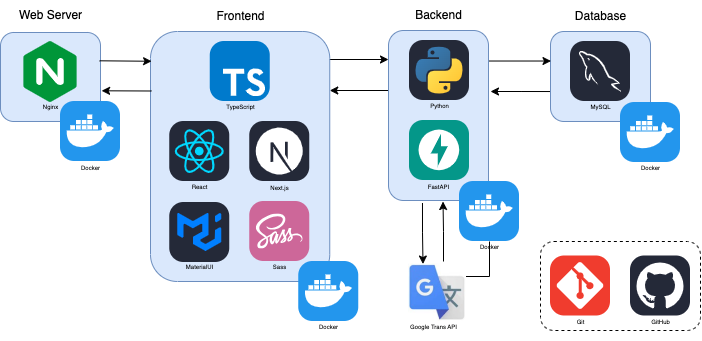
\includegraphics[width=100mm,height=48.58mm]{./img/system/technology_stack.png}
	\caption{技術スタック図}
	\label{fig:tech_stack}
\end{figure}


\subsection{サーバー}
本研究では,さくらのVPSをサーバーとして使用している.サーバーのオペレーティングシステムにはUbuntu 22.04.3 LTSを採用した.以下にサーバーのCPU,メモリ,ストレージ,ネットワークインターフェイスに関する詳細な情報を記載する.


\subsubsection{メモリ情報}
サーバーのメモリは以下の通りである.
\begin{itemize}
    \item \textbf{合計}: 7937 MB
    \item \textbf{使用中}: 1534 MB
    \item \textbf{空き}: 860 MB
    \item \textbf{バッファ/キャッシュ}: 5541 MB
    \item \textbf{利用可能}: 6094 MB
    \item \textbf{スワップ}: 0 MB
\end{itemize}


\subsubsection{ディスク使用状況}
サーバーのディスク使用状況は以下の通りである.
\begin{itemize}
    \item \textbf{ファイルシステム}:
    \begin{itemize}
        \item \textbf{tmpfs}: 使用中794 MB(使用中1.4 MB,空き793 MB)
        \item \textbf{/dev/vda2}: 使用中788 GB(使用中40 GB,空き708 GB)
    \end{itemize}
\end{itemize}


\subsubsection{ディスク構成}
サーバーのディスク構成は以下の通りである.
\begin{itemize}
    \item \textbf{ディスク名}: vda
    \item \textbf{サイズ}: 800 GB
    \item \textbf{タイプ}: ディスク
    \item \textbf{パーティション}:
    \begin{itemize}
        \item \textbf{vda1}: 1 MB
        \item \textbf{vda2}: 800 GB(マウントポイント: /)
    \end{itemize}
\end{itemize}


\subsubsection{CPU情報}
サーバーのCPUに関する情報は以下のとおりである.
\begin{itemize}
    \item \textbf{アーキテクチャ}: x86\_64
    \item \textbf{CPU 操作モード}: 32-bit,64-bit
    \item \textbf{アドレスサイズ}: 46ビット物理,48ビット仮想
    \item \textbf{バイト順序}: Little Endian

    \item \textbf{CPU総数}: 6
    \item \textbf{オンラインCPUリスト}: 0-5
    \item \textbf{ベンダーID}: GenuineIntel
    \item \textbf{モデル名}: Intel Xeon Processor (Cascadelake)
    \item \textbf{CPUファミリー}: 6
    \item \textbf{モデル}: 85
    \item \textbf{コアあたりのスレッド数}: 1
    \item \textbf{ソケットあたりのコア数}: 1
    \item \textbf{ソケット数}: 6
    \item \textbf{ステッピング}: 5
    \item \textbf{BogoMIPS}: 4199.99
    \item \textbf{サポートされているフラグ}: [フラグのリスト]

    \item \textbf{ハイパーバイザのベンダー}: KVM
    \item \textbf{仮想化タイプ}: 完全仮想化

    \item \textbf{キャッシュの合計}:
        \begin{itemize}
            \item L1d: 192KiB (6インスタンス)
            \item L1i: 192KiB (6インスタンス)
            \item L2: 24MiB (6インスタンス)
        \end{itemize}

    \item \textbf{NUMAノード数}: 1
    \item \textbf{NUMAノード0 CPU}: 0-5

    \item \textbf{脆弱性と軽減策}:
        \begin{itemize}
            \item L1tf: PTE Inversionによる軽減
            \item Meltdown: PTIによる軽減
            \item Spectre v1: ユーザーコピー/swapgsバリア,ユーザーポインターのサニタイズによる軽減
            \item Spectre v2: IBRS,IBPB条件付き,STIBP無効,RSB充填,PBRSB-eIBRS Not affectedによる軽減
        \end{itemize}
\end{itemize}


\subsubsection{ネットワークインターフェイスの状態}
サーバーのネットワークインターフェイスの設定と状態は以下の通りである.
\begin{itemize}
    \item \textbf{br-f4387cc8d030}:
    \begin{itemize}
        \item IPアドレス: 172.18.0.1/16
        \item MACアドレス: 02:42:06:18:81:07
        \item 受信パケット: 851,033 (2.0 GB)
        \item 送信パケット: 893,012 (78.0 MB)
    \end{itemize}

    \item \textbf{docker0}:
    \begin{itemize}
        \item IPアドレス: 172.17.0.1/16
        \item MACアドレス: 02:42:bf:a4:bf:64
        \item 受信パケット: 6,763 (625.9 KB)
        \item 送信パケット: 7,761 (43.2 MB)
    \end{itemize}
\end{itemize}


\subsection{セキュリティ対策}

本研究では,システムのセキュリティ強化のためにファイアウォール(UFW)とAIDE(Advanced Intrusion Detection Environment)を導入した.

\subsubsection{ファイアウォール(UFW)の設定}
本システムでは,外部からの不正アクセスを防ぎ,内部ネットワークのセキュリティを高めるためにファイアウォール(UFW)を設定している.ファイアウォールは,不正なネットワークトラフィックを検出しブロックすることで,システムを保護する重要なセキュリティ機能である.以下がその具体的な設定である.

\begin{itemize}
    \item \textbf{状態}: アクティブ
    \item \textbf{ルール}:
    \begin{itemize}
        \item \textbf{ポート 22/tcp}: 全てのアドレスからのアクセスを許可
        \item \textbf{ポート 443/tcp}: 全てのアドレスからのアクセスを許可
        \item IPv6に関しても同様の設定
    \end{itemize}
\end{itemize}

このように設定することで,システムは不正なアクセスを効果的に阻止し,同時に必要な通信は許可することができる.結果として,セキュリティを損なうことなく,システムの柔軟性とアクセシビリティを維持している.


\subsubsection{AIDE(Advanced Intrusion Detection Environment)の導入}
本システムでは,ファイルシステムの整合性を監視するためにAIDEを使用している.AIDEはファイル変更を検出するホストベースの侵入検出システムで,システムに不正な変更が生じた場合に警告を発する.

AIDEの設定は以下の通り.
\begin{itemize}
    \item AIDEのスケジュール設定:システムは毎日午前0時にAIDEを実行し,ファイルシステムの整合性をチェックする.
    \item メール通知の設定:異常が検出された場合,システムは自動的に指定したE-mailアドレスに通知する.
\end{itemize}
このセットアップにより,システムの安全性を高め,不正アクセスや変更があった場合に迅速に対応できる.


\subsection{バックエンド開発}
本研究のバックエンド開発においては,Python言語とFastAPIフレームワークを中心に,多様なライブラリを利用した.Pythonはバックエンドの主要言語として,FastAPIは主要フレームワークとして採用した.また,翻訳機能はgoogletransライブラリを用いて実現した.

以下に,本研究において使用したライブラリの一覧を示す.
\begin{itemize}
    \item anyio: 3.6.2
    \item cachetools: 5.3.1
    \item certifi: 2022.12.7
    \item chardet: 3.0.4
    \item click: 8.1.3
    \item fastapi: 0.95.1
    \item googletrans: 4.0.0rc1
    \item h11: 0.9.0
    \item h2: 3.2.0
    \item hpack: 3.0.0
    \item hstspreload: 2023.1.1
    \item httpcore: 0.9.1
    \item httptools: 0.5.0
    \item httpx: 0.13.3
    \item hyperframe: 5.2.0
    \item idna: 2.10
    \item mysql: 0.0.3
    \item mysql-connector-python: 8.0.33
    \item mysqlclient: 2.1.1
    \item protobuf: 3.20.3
    \item pydantic: 1.10.7
    \item python-dotenv: 1.0.0
    \item pytz: 2023.3
    \item PyYAML: 6.0
    \item rfc3986: 1.5.0
    \item sniffio: 1.3.0
    \item starlette: 0.26.1
    \item typing\_extensions: 4.5.0
    \item uvicorn: 0.22.0
    \item uvloop: 0.17.0
    \item watchfiles: 0.19.0
    \item websockets: 11.0.2
\end{itemize}


\subsection{フロントエンド開発}
本研究のフロントエンド開発においては,TypeScript言語とReactライブラリ,Next.jsフレームワークを中心に,Material UIを含む多様なライブラリを利用した.TypeScriptはフロントエンドの主要言語として,ReactとNext.jsは主要なライブラリとフレームワークとして採用した.また,UIコンポーネントはMaterial UIを用いて実現した.


\subsubsection{依存関係}
フロントエンド開発において直接利用されたライブラリの一覧を示す.

\begin{itemize}
    \item @emotion/react: 11.11.0
    \item @emotion/styled: 11.11.0
    \item @mui/icons-material: 5.11.16
    \item @mui/material: 5.13.2
    \item @types/gtag.js: 0.0.17
    \item @types/js-cookie: 3.0.3
    \item @types/moment: 2.13.0
    \item js-cookie: 3.0.5
    \item moment: 2.29.4
    \item moment-timezone: 0.5.43
    \item next: 13.3.1
    \item next-sitemap: 4.2.3
    \item normalize.css: 8.0.1
    \item react: 18.2.0
    \item react-dom: 18.2.0
    \item react-hook-form: 7.45.2
    \item sass: 1.62.1
\end{itemize}


\subsubsection{開発用依存関係}
開発プロセスを支援するために使用されたライブラリの一覧を示す.

\begin{itemize}
    \item @types/node: 18.16.0
    \item @types/react: 18.0.38
    \item @types/react-dom: 18.0.11
    \item @typescript-eslint/eslint-plugin: 5.59.0
    \item @typescript-eslint/parser: 5.59.0
    \item eslint: 8.39.0
    \item eslint-config-next: 13.3.1
    \item eslint-config-prettier: 8.8.0
    \item eslint-plugin-prettier: 4.2.1
    \item prettier: 2.8.8
    \item typescript: 5.0.4
\end{itemize}
% \subsection{フロントエンドについて}
% フロントエンドの開発には,特定のライブラリとツールが利用されている.このセクションでは,これらの技術の選択とそれらがインターフェイス構築や機能開発にどのように貢献するかについて述べる.ここにライブラリの詳細を書き並べる.


\subsection{データベースについて}
本研究のデータベースには,MySQL(8.0.1)を採用した.


\subsection{通信の取り扱いとNginxの役割}
本研究で使用されたWebサーバーNginxの設定は,セキュリティを重視した基準に基づいて行われている.この設定は,通信の安全性を確保しつつ,ユーザーのリクエストを効率的に処理することを目的としている.

\subsubsection{通信プロトコルの変更}
システムは公開初期にはHTTP通信を採用していたが,セキュリティの向上を目的としてHTTPS通信への移行を行った.この移行に伴い,NginxにはHTTPからHTTPSへの自動リダイレクト設定が追加された.これにより,ユーザーがHTTPでアクセスした際には,安全なHTTPS通信へと自動的に転送されるようにしている.

\subsubsection{プロキシとリバースプロキシの設定}
Nginxは,フロントエンドとバックエンド間のリクエスト転送を効率化するプロキシおよびリバースプロキシサーバーとして機能している.具体的には,ユーザーがフロントエンドにアクセスする際にNginxを経由し,必要なデータの取得を行う.また,ユーザーからのPOSTリクエストはNginxを通じてバックエンドに転送され,処理される.

% 本システムにおける通信はhttpsを通じて行われ,セキュリティを確保しつつユーザーのリクエストを効率的に処理する.ユーザーは初めにNginxを経由してフロントエンドの画面にアクセスし,画面表示に必要なデータを取得する.また,ユーザーからのPOSTアクセスはNginxを通じてバックエンドに転送され,処理される.このセクションでは,Nginxがシステム内で果たす重要な役割と,それが通信プロセスにどのように統合されているかについて詳述する.


\section{コンポーネント設計}
この掲示板システムは,表示コンポーネント及びデータ更新コンポーネントという二つの主要な構成要素から成立している.表示コンポーネントは,ユーザーインターフェースとして機能するブラウザとの通信を担当し,データ取得時にユーザーの言語情報を収集する.これにより,ユーザーの言語に応じた適切なデータをブラウザに表示する.一方,データ更新コンポーネントは,主にユーザーによる投稿データの更新を管理する.このコンポーネントは,ブラウザから送信されるデータの検証と処理を行い,その後,データベースにデータを保存する.これにより,ユーザーのインタラクションに基づく動的なコンテンツの生成と管理が可能となる.
% この掲示板は,表示コンポーネント,データ更新コンポーネントからなる.ユーザー側インターフェイスであるブラウザと通信するのは表示コンポーネントである.表示コンポーネントはデータを取得する際,ユーザーの言語の情報を付随させ,ユーザーの言語に合わせたデータをブラウザに表示する.
% データ更新コンポーネントは,主にユーザーの投稿によるデータの更新を行う.ブラウザから送られてくるデータのバリデーションや適切な処理を行い,データベースに保存する.


% 表示コンポーネント(ページ,ページ固有データ,データ取得,API)
% データ更新コンポーネント(ページ,API,router, application, infrastructure, detabase)
% この掲示板は,表示コンポーネント,データ取得コンポーネント,データ更新コンポーネントからなる.ユーザー側インターフェイスであるWebブラウザと通信するのは表示コンポーネントである.表示コンポーネントは,画面を表示するために必要なデータをデータ取得コンポーネントに要求する.データ取得コンポーネントは,その要求を読み取り,適切に加工されたデータを表示コンポーネントに渡す.また,表示コンポーネントは,ユーザーのスレッド作成やコメント投稿に応じてデータ更新コンポーネントを呼び出し,処理を要求する.データ取得コンポーネントはその要求を読み取り,データを適切に加工して保存する.

% 動的な文章の翻訳はデータ取得コンポーネントで行なっている.表示コンポーネントがデータ取得コンポーネントに処理を要求する際,ユーザーが選択している言語の情報を付属させる.データ取得コンポーネントはデータを取得した後,その言語に翻訳を行い表示コンポーネントにデータを渡す.さらに,システムは翻訳の高速化と効率化のためにキャッシュ機能を実装している.一度翻訳された文章はキャッシュに保存され,同じ文章の再翻訳が必要な場合,システムはキャッシュから翻訳済みのデータを読み込む.これにより,翻訳のたびに新たに翻訳を行う必要がなくなり,システムの応答時間を大幅に短縮できる.このキャッシュシステムは,特に多言語での交流が活発な掲示板において,ユーザー体験の向上に大きく寄与している.


\section{コンポーネントの詳細}


\subsection*{表示コンポーネント}

表示コンポーネントは,ユーザーインターフェイスの構成要素として機能し,以下のファイル構造によって定義されている.

ウェブページは,それぞれ独立したファイルによって構築される.

\begin{itemize}
\item \texttt{/pages/index.tsx} ― トップページ
\item \texttt{/pages/policy.tsx} ― プライバシーポリシーページ
\item \texttt{/pages/terms.tsx} ― 利用規約ページ
\item \texttt{/pages/404.tsx} ― 404エラーページ
\item \texttt{/pages/thread/create.tsx} ― スレッド作成ページ
\item \texttt{/pages/thread/index.tsx} ― スレッド詳細ページ
\end{itemize}

UIコンポーネントは再利用性を考慮して設計され,AtomsおよびOrganismsの二つのカテゴリに分類される.Atomsは単純なUI要素を,Organismsは複数のAtoms要素を組み合わせて構成されるより複雑なUIセクションを形成する.

Atomsカテゴリには以下のコンポーネントが含まれる.

\begin{itemize}
    \item \texttt{CustomTextField.tsx} ― ユーザー入力を受け取るフィールド
    \item \texttt{MenuListItem.tsx} ― メニュー項目表示
    \item \texttt{TextWithNewLines.tsx} ― 改行を含むテキスト表示
\end{itemize}

Organismsカテゴリは以下のコンポーネントを含む.

\begin{itemize}
    \item \texttt{CookieBanner.tsx} ― クッキーの使用に関するユーザーへの通知バナー表示
    \item \texttt{Footer.tsx} ― フッター表示
    \item \texttt{Header.tsx} ― ヘッダー表示
    \item \texttt{Meta.tsx} ― ウェブページのメタデータ
    \item \texttt{Pager.tsx} ― ページャー表示
    \item \texttt{ThreadList.tsx} ― スレッドリスト表示
\end{itemize}

図\ref{display_component_sequence_diagram}は,表示コンポーネントの動作プロセスを示したシーケンス図である.

(1)
ブラウザはサーバーに対し,ページ固有データの要求を行う.ページ固有データには,ページタイトル,ボタンのラベル,利用規約,免責事項といった静的情報が含まれている.これらの情報は多言語に対応しており,ブラウザ及びユーザーの言語設定に基づいて提供される.翻訳APIを使用しないことにより,システムの処理時間の短縮が図られている.ページ固有データの取得後,ブラウザは画面を構築し,ユーザーに対して表示を行う.

(2)
ブラウザは,ページ表示のための動的データをサーバーに要求する.動的データが取得されるまでの間,スケルトンスクリーンを用いて表示がなされる(図参照).プロセス(3)および(4)が完了すると,ページデータがブラウザに返送される.

(3)
サーバーは,ブラウザからのリクエストを解析し,データベースからデータを取得する.取得したデータはブラウザに返す形式に変換される.

(4)
サーバーは,ブラウザの選択した言語情報に従って内容を翻訳する.そのために外部の翻訳APIにリクエストを送信し,返された翻訳結果をブラウザに返す.



\newpage

\begin{figure}[H]
    \centering
    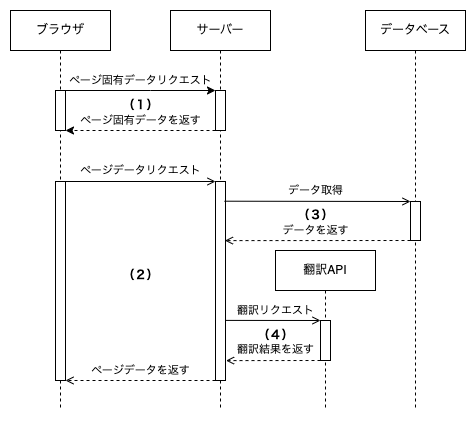
\includegraphics[width=120mm,height=110mm]{./img/components/display_component_sequence_diagram.png}
    \caption{表示コンポーネントのシーケンス図}
    \label{display_component_sequence_diagram}
\end{figure}


% \section{コンポーネントの詳細}


% \subsection*{表示コンポーネント}

% 表示コンポーネントは,ユーザーインターフェイスの構成要素であり,次のようなファイル構造を持つ.

% ウェブページは,それぞれ特定のファイルで定義される.

% \begin{itemize}
% \item \texttt{/pages/index.tsx} … トップページ
% \item \texttt{/pages/policy.tsx} … プライバシーポリシーページ
% \item \texttt{/pages/terms.tsx} … 利用規約ページ
% \item \texttt{/pages/404.tsx} … 404エラーページ
% \item \texttt{/pages/thread/create.tsx} … スレッド作成ページ
% \item \texttt{/pages/thread/index.tsx} … スレッド一覧ページ
% \end{itemize}

% さらに,再利用可能なUIコンポーネントはAtomsとOrganismsの二つのカテゴリに整理されている.Atomsは基本的なUI要素を,Organismsはこれら基本要素を組み合わせてより複雑なUIセクションを構築するための要素を含む.

% Atomsカテゴリには,次のようなコンポーネントがある.

% \begin{itemize}
% \item \texttt{CustomTextField/CustomTextField.tsx} … 入力フィールドのカスタマイズ
% \item \texttt{MenuListItem/MenuListItem.tsx} … メニュー項目のリスト表示
% \item \texttt{TextWithNewLines/TextWithNewLines.tsx} … 改行を含むテキストの表示
% \end{itemize}

% Organismsカテゴリには,次のコンポーネントが含まれる.

% \begin{itemize}
% \item \texttt{CookieBanner/CookieBanner.tsx} … クッキー利用に関する通知バナー
% \item \texttt{Footer/Footer.tsx} … ウェブページのフッター
% \item \texttt{Header/Header.tsx} … ウェブページのヘッダー
% \item \texttt{Meta/Meta.tsx} … ページのメタ情報を扱う
% \item \texttt{Pager/Pager.tsx} … ページ間のナビゲーションを提供
% \item \texttt{ThreadList/ThreadList.tsx} … スレッドの一覧表示
% \end{itemize}

% これらのコンポーネントは,ウェブアプリケーションの柔軟性と再利用性を向上させるために,体系的に分類されている.

% 本図は,表示コンポーネントの動作を示すシーケンス図である.

% プロセスは,ブラウザがサーバーに対してページ固有データを要求することから始まる.ページ固有データとは,ページタイトル,ボタンのラベル,利用規約,免責事項といった,ユーザーの操作に依存しない静的情報である.これらは複数の言語に対応しており,ブラウザとユーザーの言語選択に基づいて適切に提供される.翻訳APIを介さずにページ固有のテキストを提供することで,システムの処理時間が削減される.ページ固有データの取得後,ブラウザにより画面が構築される.

% 続いて,ブラウザはサーバーに対してページ表示に必要な動的データの要求を行う.サーバーはこの要求に応じてデータベースから該当データを抽出し,ユーザーの言語選択に沿って翻訳APIで翻訳を行う.翻訳されたデータはブラウザに送信され,最終的にユーザーに表示される.


% % \newpage
% \begin{figure}[H]
% 	\centering
% 	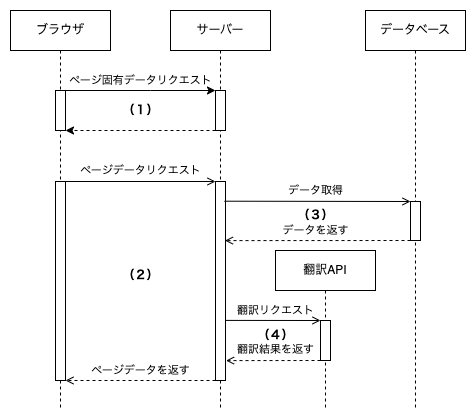
\includegraphics[width=120mm,height=110mm]{./img/display_component_sequence_diagram.png}
% 	\caption{シーケンス図}
% 	% \label{fig:tech_stack}
% \end{figure}

% \red{// TODO: 表示の流れの図}

% 図は,画面表示の際の表示コンポーネントの振る舞いをあらわしたものである.表示コンポーネントは,それぞれページとそのページで使用される部品であるコンポーネントから成り立っている.また,画像やアイコンに関して専用のpublicフォルダを用意し,そこから読み込んでいる.

\subsection*{データ更新コンポーネント}

データ更新コンポーネントは以下のような構成になっている.

\begin{itemize}
    \item \texttt{thread\_router.py} … スレッド関連のルーティングを管理
    \item \texttt{thread\_application.py} … スレッドのアプリケーションロジックを処理
    \item \texttt{thread\_infrastructure.py} … スレッドのインフラストラクチャ関連処理
    \item \texttt{comment\_router.py} … コメント関連のルーティングを管理
    \item \texttt{comment\_application.py} … コメントのアプリケーションロジックを処理
    \item \texttt{comment\_infrastructure.py} … コメントのインフラストラクチャ関連処理
    \item \texttt{translation.py} … 翻訳機能の実装
\end{itemize}

% \red{// TODO: データ更新の流れの図}

上記のファイルリストは,以下のアーキテクチャを採用し作成された.このアーキテクチャは,役割と責任を持つ複数のレイヤーに分かれている.

\paragraph{ルーターレイヤー}\mbox{}\\
\texttt{thread\_router.py} と \texttt{comment\_router.py} はルーターレイヤーに属し,外部からのリクエストを適切な処理ロジックに振り分ける役割を担う.このレイヤーは,リクエストの初期解析とルーティングを行い,システムの入口点として機能する.

\paragraph{アプリケーションロジックレイヤー}\mbox{}\\
\texttt{thread\_application.py} と \texttt{comment\_application.py} はアプリケーションロジックレイヤーを構成し,スレッドとコメントに関するビジネスロジックを実装する.このレイヤーは,アプリケーションの核心的な機能を担い,データの処理やビジネスルールの適用を行う.

\paragraph{インフラストラクチャレイヤー}\mbox{}\\
\texttt{thread\_infrastructure.py} と \texttt{comment\_infrastructure.py} はインフラストラクチャレイヤーに属し,データベースとのやり取りやデータの永続化を管理する.このレイヤーは,システムのデータ層に関わる処理を担当し,データの整合性と安全性を保証する.

\paragraph{翻訳機能}\mbox{}\\
\texttt{translation.py} は,これらのレイヤーとは別に,システム全体の翻訳機能を提供する.このファイルは,多言語サポートを実現し,異なる言語間でのコミュニケーションを可能にする.

以上のように,各レイヤーは特定の役割を持ち,システム全体の効率的かつ整理された運用を支援する.このレイヤー化されたアーキテクチャにより,システムの拡張性,保守性,およびスケーラビリティが向上している.


図\ref{data_update_component_sequence_diagram}は,データ更新コンポーネントの動作プロセスを示したシーケンス図である.

(1)ブラウザは,データ更新のためのリクエストをサーバーに送信する.このリクエストには,ユーザーが行ったデータ変更の要求が含まれており,サーバーはこれを受け取って処理を開始する.

(2)サーバーは,ブラウザからの要求に基づいてデータベースに更新を行うためのクエリを発行する.この際,データベースは更新を行い,その結果をサーバーに返送する.

(3)サーバーは,データベースから受け取った結果をブラウザが解釈できる形式に変換し,ブラウザに送信する.これにより,ブラウザはデータ更新をユーザーに対して反映する.

(4)最後に,ブラウザは更新されたデータをユーザーインターフェイスに表示し,ユーザーが最新の情報を閲覧できるようにする.

% \newpag

\begin{figure}[H]
    \centering
    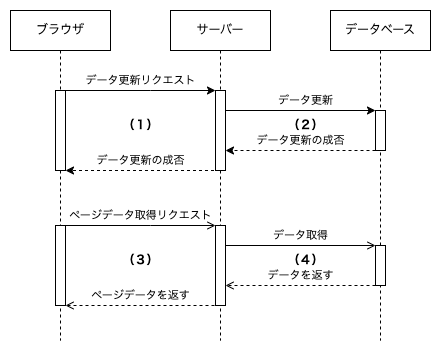
\includegraphics[width=\textwidth]{./img/components/data_update_component_sequence_diagram.png}
    \caption{データ更新コンポーネントのシーケンス図}
    \label{data_update_component_sequence_diagram}
\end{figure}


\section{データ設計}

\subsection*{Threadsテーブル}

スレッドの情報を格納するテーブルである.

\begin{table}[H]
    \centering
    \caption{スレッド情報テーブル}
    \begin{tabular}{|l|l|l|}
        \hline
        \textbf{カラム名} & \textbf{データ型} & \textbf{説明} \\
        \hline
        ThreadID   & INT PRIMARY KEY AUTO\_INCREMENT & スレッドのID \\
        Title      & VARCHAR(255) & スレッドのタイトル \\
        CreatedAt  & TIMESTAMP & 作成日時 \\
        UpdatedAt  & TIMESTAMP & 更新日時 \\
        UserName   & VARCHAR(255) & ユーザー名 \\
        Content    & LONGTEXT & 内容 \\
        Language   & VARCHAR(8) & 言語 \\
        \hline
    \end{tabular}
\end{table}

\subsection*{Commentsテーブル}

スレッドに投稿されたコメントを格納するテーブルである.

\begin{table}[H]
    \centering
    \caption{コメント情報テーブル}
    \begin{tabular}{|l|l|l|}
        \hline
        \textbf{カラム名} & \textbf{データ型} & \textbf{説明} \\
        \hline
        CommentID  & INT PRIMARY KEY AUTO\_INCREMENT & コメントID \\
        ThreadID   & INT & スレッドID \\
        UserName   & VARCHAR(255) & ユーザー名 \\
        Content    & TEXT & コメント内容 \\
        CreatedAt  & TIMESTAMP & 作成日時 \\
        Language   & VARCHAR(8) & 言語 \\
        \hline
    \end{tabular}
\end{table}

\subsection*{Cookieの使用について}

本システムでは,ユーザー体験の向上を目的として2種類のCookieを使用している.これらは以下の目的で利用されている.

\paragraph{「SelectedLanguage」言語設定の記録}\mbox{}\\
最後に選択した言語設定を記録する.この情報は次回のウェブサイト訪問時に参照され,以前に選択された言語で画面が表示されるようになる.これにより,ユーザーは毎回言語を選択する手間を省くことができ,より効率的かつ快適にシステムを利用可能となる.

\paragraph{「cookieAccepted」Cookie同意状態の記録}\mbox{}\\
ユーザーがCookieの使用に同意したか否かを記録する.これにより,Cookieの使用に関する通知バナーを初回訪問時のみ表示し,再訪問時には表示しないようにすることが可能となる.


\chapter{利活用についての分析}

\section{ユーザー獲得}

本研究で開発された多言語自動翻訳掲示板システム「The Channel」の利活用について分析するためには,ユーザーに使用してもらうことが必要であった.このシステムは,異なる文化や言語背景を持つユーザーが交流し,情報を共有するためのプラットフォームとして機能することを目的としている.従って,多様なユーザーを獲得し,継続的に参加を促すことが重要であった.

システムの普及に際して,ソーシャルメディアが重要な役割を担う.本研究では,Twitterを用いてシステムの普及を図った.Twitterは広範なユーザーネットワークを有し,迅速な情報伝播が可能であるため,新しいテクノロジーの告知に適したプラットフォームである.このアプローチにより,ターゲットオーディエンスに直接アピールし,関心を引きつけることが期待される.

\section{利活用の結果}
本システムの利用状況を分析するために,スレッドとコメントの言語を分析した.

\subsection{投稿}

ユーザーにより作成されたスレッドの言語分布を表\ref{tab:thread-language}に示す.スレッドの言語はGoogle Translate APIを用いて特定した.全体として25のスレッドが作成され,その内容は食べ物,アニメ,日本に関する推薦,掲示板機能の試用,豆知識,災害情報など多岐にわたった.


\begin{table}[H]
    \centering
    \caption{言語別スレッド数}
    \label{tab:thread-language}
    \begin{tabular}{|l|r|}
        \hline
        \textbf{言語} & \textbf{スレッド数} \\ \hline
        日本語       & 20               \\
        英語         & 3                 \\
        フランス語    & 1                 \\
        中国語       & 1                 \\ \hline
    \end{tabular}
\end{table}

コメントの言語分布を表\ref{tab:language-detection}に示す.これらもGoogle Translate APIを用いて言語を特定した.URLのみの投稿は言語が特定できないため,表の数字には加算していない.合計70件のコメントが投稿された.コメント内容はスレッドの内容に対する解答のようなものが大半を占めており,ユーザー間の対話は限定的だった.


\begin{table}[H]
    \centering
    \caption{言語別コメント数}
    \label{tab:language-detection}
    \begin{tabular}{|l|r|}
        \hline
        \textbf{言語} & \textbf{コメント数} \\ \hline
        日本語       & 47           \\
        英語         & 7             \\
        中国語(簡体字) & 4             \\
        中国語(繁体字) & 4             \\ 
        アラビア語     & 3             \\
        フランス語     & 1             \\
        ヨルバ語       & 1             \\
        ペルシャ語     & 1             \\
        ズールー語     & 1             \\\hline
    \end{tabular}
\end{table}

\subsection{ユーザー分析}
表\ref{table:user-by-country}は国別のユーザー数を示したものである.日本,中国,アメリカ,スペイン,インドネシアなどの国からユーザーのアクセスがあった.

\begin{table}[H]
    \centering
    \caption{国別ユーザー数}
    \label{table:user-by-country}
    \begin{tabular}{|l|r|}
        \hline
        \textbf{国名} & \textbf{ユーザー数} \\
        \hline
        日本     & 223 \\
        中国     & 17 \\
        アメリカ & 7 \\
        スペイン & 4 \\
        インドネシア & 3 \\
        香港 & 2  \\
        フィリピン   & 2  \\
        台湾 & 2 \\
        アルジェリア   & 1 \\
        エルサルバドル   & 1 \\
        アイルランド   & 1  \\
        ノルウェー & 1  \\
        \hline
    \end{tabular}
\end{table}

\subsection{翻訳の精度と効果}
異なる言語間の会話が限定的であったため,翻訳の精度と効果についての正確な検証はできなかった.しかし,スレッドの言語ではない言語でコメントの投稿があったため,翻訳を通して異なる言語での投稿は確認された.また,一部,不明確な翻訳がなされることがあった(例:「3m」という書き込みが「父方の叔父」と翻訳された).


\section{システム利用の実際と課題}

本研究で開発された多言語自動翻訳掲示板「The Channel」は,異文化間コミュニケーションの促進を目的としていた.しかし,実際の利用状況を分析した結果,いくつかの重要な課題が明らかになった.

\subsection{ユーザー獲得と普及戦略の課題}

予想されたユーザー数の獲得は達成されず,特に日本語以外を使用するユーザーの参加は限られていた.多言語間の交流はそれほど活発ではなく,掲示板では会話ではなく単発のコメントが主となっていた.

システム普及のための宣伝活動においては,ソーシャルメディアを中心としたアプローチを採用したが,多言語ユーザーに向けた有効な広告戦略の不足や,検索エンジン最適化(SEO)の知識不足が普及の妨げとなった可能性がある.この結果,広範なユーザーベースへのアプローチが困難となり,システムの認知度の向上に至らなかった.

\subsection{インターフェースデザインとユーザー定着の問題}

本研究において掲示板のインターフェースや機能などは,日本の掲示板「5ちゃんねる」を参考に設計された.この設計は,既存のユーザーにとっては馴染み深いものであったが,新たなユーザーにとっては会話を促進するような機能やインターフェースの工夫が不足していた.結果として,ユーザー間の継続的な対話やコミュニティ形成を促す要素が限られてしまい,ユーザーの定着率に影響を与えた可能性がある.

また,ユーザーが掲示板に継続的に参加するための魅力的なアイデアや機能の欠如が,定着率の低さに繋がったと考えられる.多言語間の交流を促す掲示板という新しいコンセプトにも関わらず,ユーザーにとって十分に魅力的な機能やインセンティブを提供できていなかった.

\subsection{開発プロセスと時間管理の問題}

本システムの開発は,著者一人で行ったため,多大な時間が費やされた.その結果,利用者獲得に向けた活動に十分な時間を割くことができず,普及戦略の展開に影響を与えた.

また,掲示板を公開してからの運用期間の短さも影響を与えている可能性がある.「2ちゃんねるには2ちゃんねる語やアスキーアートによる定型的固有表現があるが,これを使うことによって2ちゃんねるの参加者は2ちゃんねるに参加していることを潜在的にせよ強く意識する」(松村ほか,2004)ことが指摘されている.このような文化は長い時間をかけてユーザーの間で育まれていくものである.しかし,本掲示板は公開から分析までの期間は3ヶ月ほどしかなかった.そのため,このようなユーザーが定着するための文化は生まれなかった.

\section{総括と展望}

本研究で開発された「The Channel」という多言語自動翻訳掲示板は、異なる文化や言語を持つユーザー間の交流を促進することを目指していた。しかし、ソーシャルメディアを通じた宣伝活動において、期待したほどの多言語ユーザーの獲得や活発な交流には至らなかった。これは、新規ユーザーにとって魅力的な機能が不足していたり、参加を促すコミュニティ文化の育成が不十分だったことが原因であるのではないだろうか。
% さらに、翻訳技術の現在の限界と、開発および普及活動に割り当てられた時間の制約が、システムの普及に影響を与えたと推測している。

これらの経験を踏まえ、今後の掲示板システムにおける改善点として、より効果的なユーザー獲得アプローチの開発、ユーザビリティの向上、翻訳精度の改善、コミュニティ文化の育成などが挙げられる。また、より長期的な運用と詳細な評価を行うことで、システムの効果と改善策をより適切に把握し、適用することが必要である。

最後に、本研究は異文化間コミュニケーションの支援という新たな試みを提示した。将来の研究者や開発者がこれらの課題に取り組み、言語と文化の多様性を豊かにするためのプラットフォームを創出していくことを期待している。



% \section{システム利用の実際と課題}

% 本研究における多言語自動翻訳掲示板「The Channel」の開発は,異文化間コミュニケーションの促進を目指したものであった.しかし,実際の利用状況を分析すると,いくつかの重要な課題が明らかになった.

% \subsection{ユーザー獲得と普及戦略}

% まず,予期していたユーザーの獲得は実現せず,特に日本語以外の言語を用いる利用者の参加は限定的であった.多言語間の交流は活発ではなく,掲示板上では単発のコメントが主流を占めていた.

% システムの普及のための宣伝活動では,Twitterなどのソーシャルメディアを主要な手段として採用したが,多言語ユーザーを対象とした効果的な広告戦略の欠如や,検索エンジン最適化に関する専門知識の不足が障壁となった可能性がある.これにより,広範な利用者層へのアプローチが困難であり,システムの認知度向上には至らなかった.

% \subsection{開発プロセスと時間管理}

% 本システムの開発は著者一人で行ったため,多くの時間を要した.その影響で,利用者獲得のための活動時間が制限された.

% \subsection{技術的制約とユーザーエクスペリエンス}

% システムは基本機能を有していたが,ユーザーインターフェースの設計や翻訳精度に問題があり,利用者体験に影響を及ぼした.特に,専門用語や俗語を含む文章では翻訳誤りが発生し,これがコミュニケーションの障害となった.

% \subsection{コミュニティ形成の課題}

% 利用者間の継続的な交流を促進する目的で開発されたが,実際には限定的な相互作用に留まり,活発なコミュニティの形成には至らなかった.交流を促進するための機能の不足,言語の障壁,文化的相違がコミュニティ形成の妨げとなった.


% これらの課題を踏まえ,今後の改善点としては,より戦略的なユーザー獲得計画の策定,利用者インターフェースの改善,翻訳精度の向上,コミュニティ構築への取り組みなどが考えられる.また,マーケティングと検索エンジン最適化に関する専門知識の向上も,プロジェクトの成功において重要である.

% これらの改善策により,「The Channel」は,異文化間の交流と理解を深めるための有力なプラットフォームへと成長することが期待される.




% \section{システム利用の実際と課題}

% 本研究における多言語自動翻訳掲示板「The Channel」の開発は,異文化間コミュニケーションの促進を目指したものであったが,実際の利用状況においていくつかの重要な課題が浮上した.

% \subsection{ユーザー獲得の難しさ}

% 予期していたほどのユーザー獲得は実現せず,特に日本語以外の言語を用いる利用者の参加は限られていた.多言語間の交流は活発でなく,掲示板上では単発のコメントや質問が主となっていた.

% \subsection{宣伝活動に関する問題点}

% システム普及のための宣伝活動では,ソーシャルメディアを主な手段としたが,多言語ユーザーを対象とした効果的な広告戦略の欠如や,検索エンジン最適化に関する専門知識の不足が障壁となった.これにより,広範な利用者層へのアプローチが困難であり,システムの認知度向上には至らなかった.

% \subsection{開発プロセスと時間管理の問題}

% 本システムの開発は個人によるものであり,多くの時間を要するプロセスであった.特に,異なる技術の統合に際して技術的な困難が発生し,利用者獲得のための活動時間が制限された.

% \subsection{技術的制約とユーザーエクスペリエンス}

% システムは基本機能を有していたが,ユーザーインターフェースの設計や翻訳精度に問題があり,利用者体験に影響を及ぼした.特に,専門用語や俗語を含む文章では翻訳誤りが発生し,これがコミュニケーションの障害となった.

% \subsection{コミュニティ形成の課題}

% 利用者間の継続的な交流の促進を目指していたが,実際には限定的な相互作用に留まり,活発なコミュニティの形成には至らなかった.交流を促進するための機能の不足や言語の障壁,文化的相違がコミュニティ形成の妨げとなった.

% \subsection{マーケティング戦略と普及計画の不備}

% 効果的なマーケティング戦略の欠如は,プロジェクトの大きな障壁となった.ターゲットオーディエンスの特定や,適切なアピール方法の欠如が,システムの普及を制限した.

% これらの課題を踏まえて,今後の改善点としては,より戦略的なユーザー獲得計画の策定,利用者インターフェースの改善,翻訳精度の向上,コミュニティ構築への取り組みなどが考えられる.また,マーケティングと検索エンジン最適化に関する専門知識の向上も,プロジェクトの成功において重要である.


% \subsection{改善策と将来的展望}

% 本研究で明らかになった課題に対処し,多言語自動翻訳掲示板「The Channel」の潜在能力を最大限に引き出すために,以下のような改善策が提案される.

% \subsubsection{戦略的ユーザー獲得計画}

% ユーザー獲得を拡大するためには,多様な文化や言語のコミュニティをターゲットとする戦略的な計画が必要である.これには,各言語・文化圏に合わせたマーケティング活動,パートナーシップの確立,イベントやコンテストの開催などが含まれる.また,異文化間交流を促進するためのユニークな機能の開発や,ユーザー参加型のコンテンツ作成も効果的である.

% \subsubsection{利用者インターフェースの改善}

% 利用者インターフェースは,直感的かつ利用しやすいものでなければならない.ユーザビリティテストを通じて,利用者のニーズに基づいたデザインの最適化を行う.また,モバイルデバイスや異なるブラウザでの利用を考慮したレスポンシブデザインの実装も重要である.

% \subsubsection{翻訳精度の向上}

% 翻訳精度の向上は,システムの核となる部分である.最新の機械翻訳技術の導入や,専門用語のデータベース構築により,翻訳の質を向上させる.また,ユーザーが翻訳を編集・改善できる機能を提供することで,コミュニティ主導の翻訳改善が可能となる.

% \subsubsection{コミュニティ構築の強化}

% 活発なコミュニティの構築には,ユーザー間の相互作用を促進する機能やイベントが必要である.フォーラムやグループ機能の導入,多文化イベントの開催などにより,ユーザーが積極的に交流する環境を作り出す.また,ユーザーのフィードバックを定期的に収集し,システム改善に反映させることが重要である.

% \subsubsection{マーケティングとSEOの専門知識の強化}

% 効果的なマーケティング戦略と検索エンジン最適化の専門知識は,プロジェクトの成功に不可欠である.これには,SNSマーケティングの強化,ターゲットオーディエンス分析,SEOに関する研修や勉強会の参加が含まれる.また,マーケティングとSEOの専門家とのコラボレーションにより,より効果的な戦略を立てることができる.

% これらの改善策により,「The Channel」は,異文化間の交流と理解を深めるための有力なプラットフォームへと成長することが期待される.




% \section{システム利用の実際と課題}

% 本研究において開発された多言語自動翻訳掲示板「The Channel」は,卒業論文のために個人で開発された.このプロジェクトの主要な目的は,異なる言語や文化を持つユーザー間の交流を促進することにあった.しかし,システムの利用においていくつかの課題が浮かび上がった.

% まず,想定していたほどのユーザーが集まらなかった.特に,日本語以外の言語でのアクティブなユーザーが少なく,多言語間での交流が限定的であった.また,システムに投稿される内容も,ユーザー同士の実質的な会話よりも,単発のコメントや質問に留まる傾向が見られた.

% システムの宣伝に関しても課題が存在した.特に,Twitterなどのソーシャルメディアを利用した宣伝活動では,ターゲットとなる多言語使用者を効果的に引き付けることが困難であった.加えて,SEO(検索エンジン最適化)やマーケティングに関する専門知識が不足していたため,より広範なユーザー層にアプローチすることが難しかった.

% さらに,開発は一人で行われたため,時間とリソースの制約が大きな問題となった.開発にかかる時間が予想以上に長引いた結果,ユーザーを集めるための時間が十分に確保できず,システムの普及が思うように進まなかった.

% これらの課題にもかかわらず,システムは基本的な機能を備え,異なる言語間での交流を可能にすることに成功した.しかし,より多くのユーザーを惹きつけ,活発なコミュニティを形成するためには,さらなる宣伝活動やユーザー体験の改善が必要であると考えられる.

% \begin{table}[H]
%     \centering
%     \begin{tabular}{|l|c|c|}
%         \hline
%         \textbf{言語ペア} & \textbf{投稿数} & \textbf{コメント数} \\
%         \hline
%         日本語 → 日本語 & 150 & 300 \\
%         日本語 → 英語   & 100 & 200 \\
%         日本語 → 中国語 & 50  & 120 \\
%         日本語 → スペイン語 & 40  & 90 \\
%         英語 → 日本語   & 100 & 180 \\
%         英語 → 英語     & 200 & 400 \\
%         英語 → 中国語   & 60  & 110 \\
%         英語 → スペイン語 & 70  & 130 \\
%         \hline
%     \end{tabular}
%     \caption{言語間コミュニケーション量\red{***データは仮置き*** 表のタイトルは上に書く}}
%     \label{table:language-communication}
% \end{table}

\begin{thebibliography}{99}

\bibitem{omukai2006} 
大向一輝 (2006). SNSの現在と展望-コミュニケーションツールから情報流通の基盤へ-. 情報処理,47(9): 993-1000.

\bibitem{ogawa2009} 
小川泰弘,福田ムフタル,外山勝彦 (2009). 日本語ーウイグル語翻訳掲示板システム. 言語処理学会 第15回年次大会発表論文集,15: 212-215.

\bibitem{kageura2017} 
影浦峡 (2017). 改めて,翻訳とは何か:Google NMTが使える時代に. 言語処理学会 第23回年次大会発表論文集,23: 931-934.

\bibitem{kameda2022} 
亀田倫史 (2022). 機械学習とバイオテクノロジー. 生物工学会誌,100(11): 588.

\bibitem{nakazawa2017} 
中澤敏明 (2017). 機械翻訳の新しいパラダイム:ニューラル機械翻訳の原理. 情報管理,60(5): 299-306.

\bibitem{notsu2009} 
野津誠 (2009). 日韓翻訳掲示板「enjoy Korea」終了へ,理由は利用率の低下. 株式会社インプレス,\url{https://internet.watch.impress.co.jp/cda/news/2009/02/12/22405.html}(参照日2023.07.17)

\bibitem{fujii2005} 
藤井薫和,重信智宏,吉野孝 (2005). 異文化間コミュニケーションのための機械翻訳を用いたチャットシステムAnnoChatの開発と適用. 情報科学技術フォーラム一般講演論文集,4(3): 437-438.

\bibitem{funakoshi2004} 
船越要,藤代祥之,野村早恵子,石田料亨 (2004). 機械翻訳を用いた協調作業支援ツールへの要求条件—日中韓馬異文化コラボレーション実験からの知見. 情報処理学会論文誌,45(1): 112-120.

% \bibitem{miyabe2009} 
% 宮部真衣,吉野孝 (2009). 折り返し翻訳を用いた翻訳リペアのチャットコミュニケーションへの影響.
\bibitem{matumura2004} 
松村真宏,三浦麻子,柴内康文,大澤幸生,石塚満 (2004). 2ちゃんねるが盛り上がるダイナミズム. 情報処理学会論文誌,45(3): 1053-1061.


\bibitem{miyabe2010} 
宮部真衣,吉野孝 (2010). 機械翻訳を介したチャットコミュニケーションにおける精度判定に基づく送信拒否の適用可能性. 情報処理学会論文誌,51(3): 784-795.

\bibitem{muramoto2022} 
村本麻衣 (2022). 自動翻訳機能からの自立:学習者による気づきを通じて. ドイツ語教育 = Deutschunterricht in Japan / 日本独文学会ドイツ語教育部会 編,26: 119-125.

\bibitem{yoshino2006} 
吉野孝,藤井薫和,重信智宏 (2006). 異文化間コミュニケーションのためのカスタマイズ可能なユーザインタフェイスを持つチャットシステムCustomChatの開発. 情報処理学会研究報告 = IPSJ SIG technical reports,(60): 13-18.

\bibitem{deepl} 
DeepL (2023). DeepL. \url{https://jobs.deepl.com/}(参照日2023.07.08)

\bibitem{googlecloud} 
Google Cloud (2023). Translation AI. \url{https://cloud.google.com/translate?hl=ja}(参照日2023.07.17)

\bibitem{loki} 
Loki Technology,Inc (2023). 5ちゃんねる. \url{https://5ch.net/}(参照日2023.07.17)

\bibitem{googletrans} 
PyPI (2023a). googletrans 3.0.0. \url{https://pypi.org/project/googletrans/}(参照日2023.07.17)

\bibitem{deeplpy} 
PyPI (2023b). deepl 1.15.0. \url{https://pypi.org/project/deepl/}(参照日2023.07.17)

\bibitem{reddit} 
Reddit Inc (2023). reddit. \url{https://www.redditinc.com/}(参照日2023.07.08)

\bibitem{server_world}
Server World (2022). AIDE : ホスト型 IDS. \url{https://www.server-world.info/query?os=Ubuntu_22.04&p=aide}(参照日2023.12.2)


\end{thebibliography}
    
% \begin{thebibliography}{99}
% % \bibitem{rika} 国立天文台編,理科年表 (丸善)
% % \bibitem{ten} 天文年鑑,誠文堂新光社.
% \end{thebibliography}

\end{document}
